\documentclass[11pt]{scrartcl}
\usepackage[utf8]{inputenc}
\usepackage[T1]{fontenc}

% Standard ams packages
\usepackage{amsmath}
\usepackage{amssymb}
\usepackage{amstext}

% Für Seitenränder
\usepackage{geometry}
\geometry{
	top=2.5cm,
	left=2.5cm,
	right=2.5cm,
	bottom=2cm,
%	includefoot,
	footskip=13.6pt
}

% Für schöneren Blocksatz
\usepackage{microtype}

% Für deutsche Sprache
\usepackage[ngerman]{babel}

% Für deutsche Zitate / Anführungszeichen
\usepackage{csquotes}

% Für Quellenangaben
\usepackage[sorting=none, defernumbers=true]{biblatex}
\addbibresource{sources.bib}

% Für klickbare links (Kasten werden nicht mitgedruckt)
\usepackage[bookmarks=true]{hyperref}
\hypersetup{
	pdftitle={Erkennung ereigniskorrelierte Potenziale eines Elektroenzephalogramms durch eine KI},
	pdfauthor={Matteo Friedrich \& Alexander Reimer},
	pdfsubject={Die Erkennung von Blinzeln in Elektroenzephalogrammen mithilfe von neuronalen Netzwerken},
	pdfkeywords={KI, AI, neuronale Netzwerke, EEG, Elektroenzephalographie, Jugend Forscht, EKP}
}

% Für Zusammenfassung
\usepackage{abstract}

% Für das Einfügen von Bildern
\usepackage{graphicx}

% Für wrapfigure (Text um Bilder herum)
\usepackage{wrapfig}

% Für Einheiten
\usepackage{siunitx}

% Für custom captions
\usepackage{caption}
\captionsetup{textfont={footnotesize}, labelfont={footnotesize, bf}, position=below, format=plain}

% Für \affil
\usepackage{authblk}

% Für Erzwingen der Abbildungs-Platzierung ([H])
\usepackage{float}

% Für Kopf-/Fußzeilen
%\usepackage{scrlayer-scrpage}
% \renewcommand*{\headfont}{\normalfont}
%\setkomafont{pagehead}
%\rehead[]{JUGEND FORSCHT -- PROJEKTBERICHT}
%\rohead[]{JUGEND FORSCHT - PROJEKTBERICHT}

\usepackage{fancyhdr}
\pagestyle{fancy}

\fancyhf{}
\fancyhead[R]{JUGEND FORSCHT -- PROJEKTBERICHT}
\fancyfoot[C]{\thepage}

% Für Seitenränder
% \usepackage{geometry}
% \geometry{left=2.5cm, right=2.5cm, top=2.5cm, bottom=2cm}

% Für schönere horizontale Linien in Tabellen
\usepackage{booktabs}

\usepackage{xurl} 

\begin{document}

	%\setlength{\footskip}{100pt}

	%\renewcommand{\footruleskip}{3cm}

	\newcommand{\sig}{\textrm{sig}}
	\newcommand{\netin}{\textrm{netzinput}}

	\newcommand{\threesub}[1]{
		\vspace{1.5ex}
		\noindent {\textbf{#1}}
		\vspace{0.5ex}
	}

	\newcommand{\form}[1]{#1}

	\newcommand{\fig}[1]{\centering #1}

	\newcommand{\filepath}[1]{\texttt{#1}}
	\newcommand{\cmd}[1]{\texttt{#1}}

	\newcommand{\ownurl}[1]{\texttt{#1}}


	% Abstand zwischen Tabellenzeilen
	\renewcommand*{\arraystretch}{1.2}


	\pagenumbering{gobble}
	\thispagestyle{empty}

	\vspace*{10mm}
	{
		\begin{center}
			\Huge \textbf{Steuerung per Lidschluss}

			Erkennung ereigniskorrelierter Potenziale eines Elektroenzephalogramms durch eine KI
			\vspace*{10mm}
		\end{center}


		\begin{center}
		
			
\includegraphics[width=0.8\textwidth]{pictures/logo.png}
		
			\vspace{15mm}
		
			{\huge \textbf{Alexander Reimer und Matteo Friedrich}}
		
			\vspace{1em}
		
			{\LARGE \textbf{Gymnasium Eversten Oldenburg}}
		
			\vspace{2em}
		
			\textbf{\Large Betreuer: Herr Dr. Glade \& Herr Husemeyer}
		\end{center}
	}






	\newpage

	\pagenumbering{arabic}
	
	\tableofcontents
	
	\newpage

	\section{Kurzfassung}


	In diesem Projekt wollen wir einen Roboter mithilfe bloßer Gedankenkraft steuern.

	Um Daten über das Gehirn zu bekommen, nutzen wir einen Elektroenzephalographen, kurz EEG, welches durch Elektroden an der Kopfhaut die Spannungsdifferenzen innerhalb des Gehirns misst. Diese werten wir mithilfe eines neuronalen Netzes aus, welches wir vorher darauf trainiert haben, Muster in diesen Daten zu erkennen. So könnte man bestimmte Ereignisse anhand der EEG-Daten ableiten, z.B. ob jemand geblinzelt hat oder sich gerade konzentriert.
	
	Das Ziel ist es dann, einen Roboter nur mit Gedanken steuern zu können.
	Wir haben bereits ein geeignetes neuronales Netz trainiert, welches Blinzeln sicher erkennen kann. 
	%Die Steuerung eines Roboters funktioniert ebenfalls.
	Daran haben wir einen Roboter gekoppelt, den wir zuverlässig über das neuronale Netz steuern können.
	Unsere Hoffnung ist, in Zukunft den Roboter auch durch Gedanken an bestimmte Richtungen und nicht nur Blinzeln steuern zu können.

	\section{Einleitung}

	Ziel des Projektes ist es, zuerst ein BCI -- Brain-Computer Interface -- zu entwickeln, welches verschiedene Ereignisse erkennen kann -- momentan, ob man gerade blinzelt. Diese Erkennung wollen wir dann zur Steuerung eines Roboters nutzen.

	BCIs sind Schnittstellen zwischen dem Gehirn und einem Computer, die eine Kommunikation vom Gehirn zum Computer ermöglichen. Man kann BCIs für die Steuerung von Prothesen, Drohnen, Robotern, und vielem mehr nutzen. \cite{bci-explained}
	Zum Beispiel haben Forscher aus Stanford ein BCI entwickelt, welches in der Lage ist, behinderten Personen die Möglichkeit zu geben, über ihre Gedanken Nachrichten zu schreiben und so kommunizieren zu können. \cite{brain2text}
	Andere Forscher haben es geschafft, Menschen mit vollständigem Locked-in-Syndrom (CLIS) mithilfe eines BCIs wieder die Kommunikation zu ermöglichen, trotz Fehlen von jeglicher willentlicher Muskelbewegungen. \cite{BCIChaudhary}
	
	Wir hoffen, bei der Erarbeitung unseres Projektes neben dem Erlangen von Erfahrung in diesem interessanten Bereich auch selbst dazu beizutragen. BCIs, die mit sehr teurer Hardware entwickelt werden, sind bereits gut erforscht. Jedoch sind diese BCIs aufgrund ihres hohen Preises für viele Konsumenten nicht interessant. Genau bei diesem Problem wollen wir mit unserem Projekt ansetzten: Wir wollen ein BCI entwickeln, welches auch mit günstiger Hardware funktioniert.
	
	Dabei ist es uns wichtig, dass unser BCI ohne spezielles Training auf eine bestimmte Person für jeden beliebigen Menschen funktioniert, und dass unser BCI auch leicht für die eigenen Zwecke anpassbar ist, z.B. die Umstellung von der Erkennung von Augenschließen zur Erkennung von Armbewegungen. Deswegen benutzen wir Open Source Software und haben unseren kompletten Code ebenfalls auf GitHub veröffentlicht.

	\section{Methode und Vorgehensweise}

	\subsection{Materialien} \label{Materialien}

	\begin{itemize}
		\item EEG
		\begin{itemize}
			\item 4 Channel Ganglion Board von OpenBCI $\star$ (s. \hyperref[Foerderverein]{Danksagung})
			\item 4x Spike und 2x Flat Electrodes  $\star$
			\item Klettband für die Elektroden $\star$
			\item 2x Earclips $\star$
			\item Lithium-Polymer-Akku und Ladegerät $\star$
			\item Plastik-Hülle für das Ganglion Board
		\end{itemize}

		\item Roboter
		\begin{itemize}
			\item Lego Mindstorms EV3 Brick
			\item Raspberry Pi 3B+ 1\,GB
			\item 2x EV3 großer Motor
			\item SD-Karte (8\,GB)
			\item diverse LEGO Teile
		\end{itemize}

		\item Computer: Aorus 15P
		\begin{itemize}
			\item CPU: i7-11800H
			\item GPU: RTX 3060
			\item RAM: 16\,GB
		\end{itemize}

		\item Software
		\begin{itemize}
			\item Julia als Programmiersprache für unser ganzes Projekt \cite{julia}
			\item Flux.jl für das neuronale Netz
				%\footnote{\href{https://github.com/FluxML/Flux.jl}{https://github.com/FluxML/Flux.jl}}
				\cite{Flux.jl-2018}
				\cite{innes:2018}
			
			\item BrainFlow.jl als Schnittstelle zum EEG
				%\footnote{\href{https://github.com/brainflow-dev/brainflow}{https://github.com/brainflow-dev/brainflow}}
				\cite{brainflow}
			
			\item FFTW.jl für die Fast Fourier Transformation
				%\footnote{\href{https://github.com/JuliaMath/FFTW.jl}{https://github.com/JuliaMath/FFTW.jl}}
				\cite{FFTW.jl-2005}
			
			\item CUDA.jl zum effektiven Nutzen einer NVIDIA GPU
				%\footnote{\href{https://github.com/JuliaGPU/CUDA.jl}{https://github.com/JuliaGPU/CUDA.jl}}
				\cite{CUDA}
			
			\item PyPlot.jl zum Plotten
				%\footnote{\href{https://github.com/JuliaPy/PyPlot.jl}{https://github.com/JuliaPy/PyPlot.jl}}
				\cite{pyplot}
			
			\item BSON.jl zum Speichern und Laden von Netzwerken
				%\footnote{\href{https://github.com/JuliaIO/BSON.jl}{https://github.com/JuliaIO/BSON.jl}}
			
			\item ev3dev als Betriebssystem auf dem EV3-Brick \cite{ev3dev-docs}
			
			\item ev3dev.jl zum Steuern eines EV3-Roboters durch einen Raspberry Pi in Julia
				%\footnote{\href{https://github.com/AR102/ev3dev.jl}{https://github.com/AR102/ev3dev.jl}}
				\cite{ev3dev}

			
		\end{itemize}

	\end{itemize}

	\begin{figure}[h!]
		\fig{
		\includegraphics[width=0.46\textwidth]{pictures/EEG-Alex-annotated.png}
		\includegraphics[width=0.3\textwidth]{pictures/Ganglion-Board-annotated.png}
		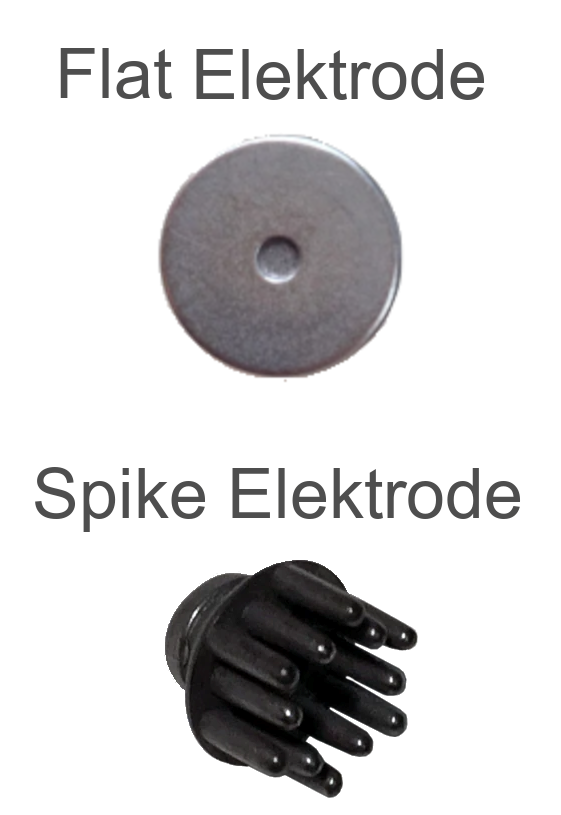
\includegraphics[width=0.15\textwidth]{pictures/spike_flat_elektroden.png}
		\caption{Das EEG und Zubehör. Links sieht man die typische Anwendung des EEG im Versuchsaufbau (Konfiguration 1, siehe Abbildung \ref{10-20-System}). In der Mitte ist das Ganglion Board genauer dargestellt. Rechts sind eine Flat Elektrode und eine Spike Elektrode zu sehen.}
		\label{EEG-Zubehor}}
	\end{figure}

	Unser EEG-Gerät besteht aus einem Klettband mit Löchern für die Elektroden, einer Platine (Ganglion Board), in welche die Elektroden eingesteckt werden, einer Kunststoff-Hülle zum Schutz des Ganglion Boards, und einem USB-Dongle, mit welchem die Signale der Platine kabellos empfangen werden können (siehe Abbildung \ref{EEG-Zubehor}).

	\subsection{Vorgehensweise}

	Unser Projekt lässt sich grob in drei Bereiche unterteilen. Zum einen gibt es den neurobiologischen Teil. Dieser besteht aus der Messung von Gehirnaktivität und der Umwandlung dieser Aktivität in für uns nutzbare Daten. Der zweite Teil besteht aus der Verarbeitung dieser Signale. Hierfür nutzen wir ein neuronales Netz, welches Muster in den Gehirnaktivitäten erkennen kann. Der letzte Teil von unserem Projekt beinhaltet die Steuerung eines EV3 Roboters. Je nachdem, was das neuronale Netz ausgibt, soll sich dieser Roboter anders verhalten und so über Gedanken steuerbar sein.	

	\subsubsection{Elektroenzephalographie}

	Bei der Elektroenzephalographie (EEG) werden Elektroden an der Kopfoberfläche platziert. Diese können sehr kleine Spannungen messen, die durch Potentialänderungen in Neuronengruppen im Gehirn entstehen und durch den Schädel dringen. Eine Elektrode kann meist nur die Summe aller lokalen Potentialänderungen messen. Man kann also auch nur ungefähr sagen, wo genau im Gehirn eine Potentialänderung stattgefunden hat. Mit mehr Elektroden kann die Genauigkeit erhöht werden. \cite{wiki:EEG} \cite{Birbaumer2010}

	Um eine Differenz bilden zu können, wird eine zweite Elektrode benötigt. Wir benutzen dafür eine Referenzelektrode, welche am Ohrläppchen befestigt wurde, wo sie ein von Gehirnströmen weitgehend unbeeinflusstes, konstantes Potential ableiten kann. Alle vier am Kopf platzierten Elektroden nutzen diese Referenzelektrode. Somit handelt es sich bei allen vieren um eine unipolare Ableitung. \cite{Praktikum}

	Wir untersuchen ereigniskorrelierte Potentiale (EKPs). Dies sind bestimmte Spannungsschwankungen (\enquote{Potentiale}), welche in Zusammenhang mit einem internen oder externen Ereignis stehen, wie z.B. einem lauten Ton, einer Körperbewegung oder hoher Konzentration. \cite{Birbaumer2010} \cite{Praktikum}
	Dabei haben wir uns zuerst für das Blinzeln entschieden, da wir es im Graphen zumindest mit bloßen Augen sehr gut erkennen konnten (siehe Abbildung \ref{EMG-Blinzeln}).

	\begin{figure}[h!]
		\fig{
		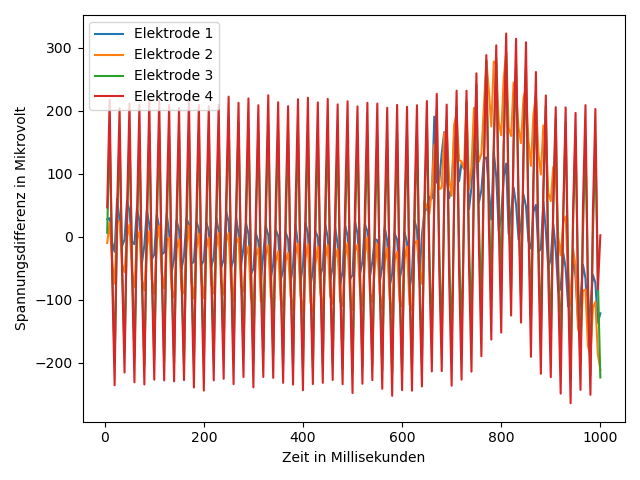
\includegraphics[width=0.8\textwidth]{pictures/EMG_blinzeln_beispiel.png}
		\caption{Ausschnitt eines EMG mit Blinzeln (Konfiguration 1).}
		\label{EMG-Blinzeln}}
	\end{figure}

	Weiter ist es möglich, nur durch Gedanken eine Steuerung auszuführen. Dies funktioniert jedoch meist durch instrumentelle oder klassische Konditionierung, also durch das Bestrafen und Belohnen auf Basis der Messungen des EEG. So kann das Gehirn darauf trainiert werden, auf Verlangen eine bestimmte, vorher festgelegte Aktivität auszulösen, die dann gemessen und ausgewertet werden kann. \cite{BCIChaudhary} Darauf wollen wir verzichten, da die Konditionierung Zeit benötigt und nicht unser Ziel einer allgemeinen Anwendbarkeit erfüllen würde.
	

	Zur Messung des EKPs haben wir zu Beginn zwei Flat Elektroden (Elektroden mit glatter Kontaktoberfläche) über den Augen und zwei Spike Elektroden (Elektroden mit langen \enquote{Spitzen}) an den Schläfen platziert (siehe Abbildung \ref{10-20-System}). Flat Elektroden haben zwar aufgrund ihrer größeren Oberfläche auf freier Haut eine etwas bessere Signalqualität, aber die von uns gewählten Stellen an den Schläfen waren leicht behaart. Die Spike Elektroden können durch die Haare leichter Kontakt zur Kopfoberfläche herstellen.

	\begin{figure}[h!]
		\fig{
		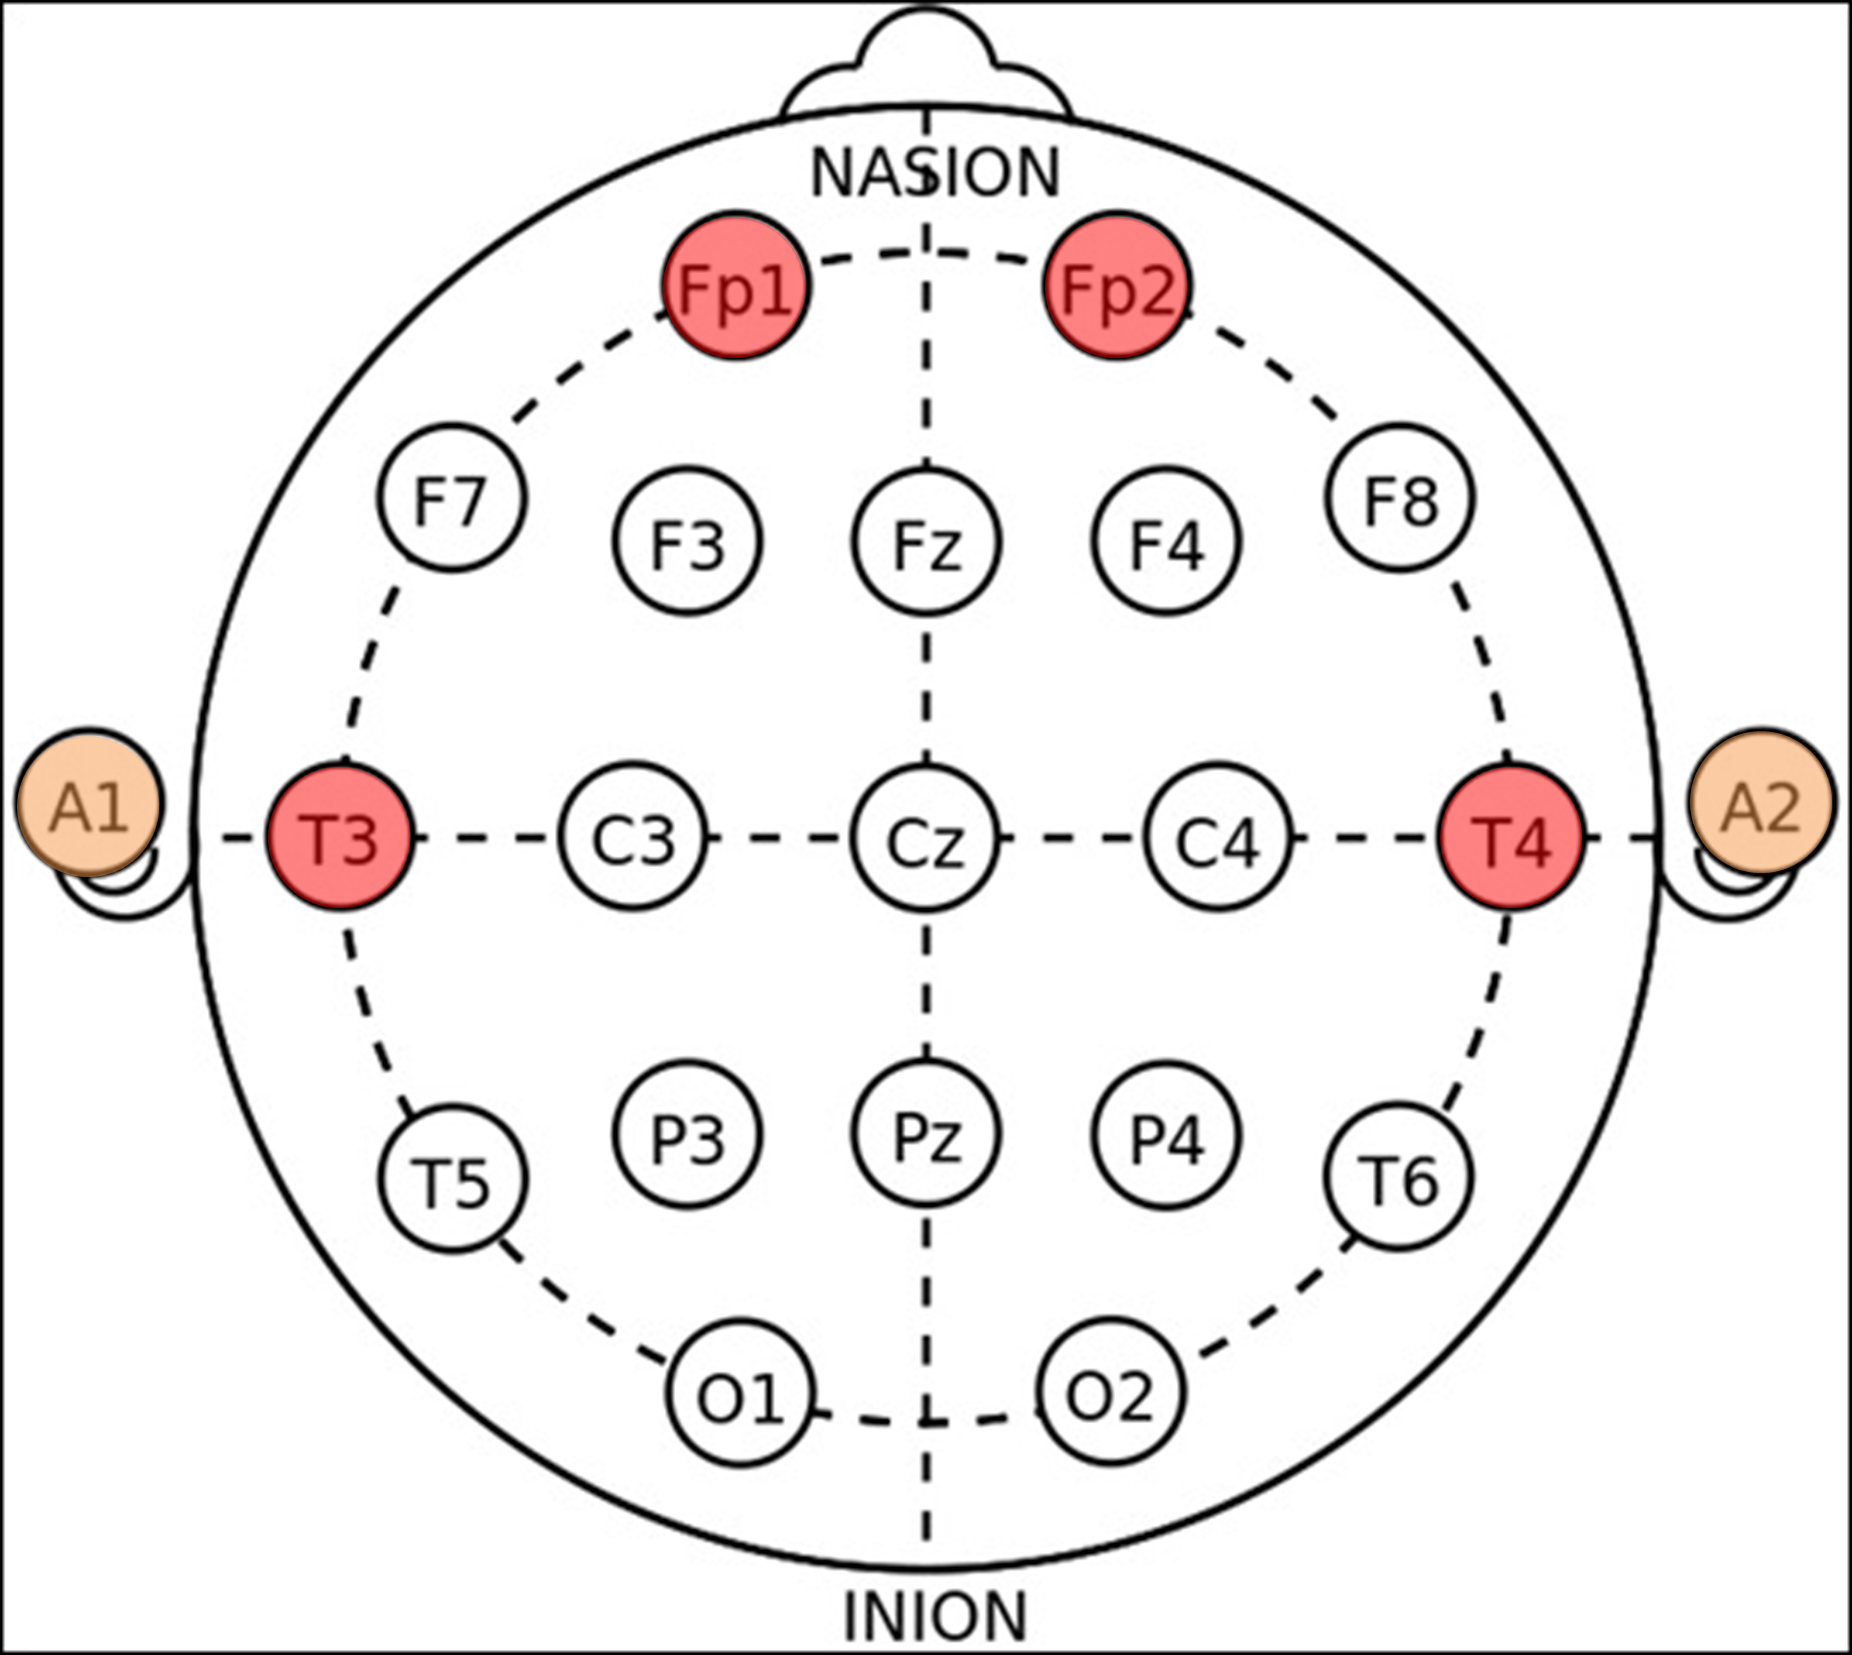
\includegraphics[width=\textwidth]{pictures/elektroden-platzierungen.png}
		\caption{10-20 System mit den von uns genutzten Flat Elektroden blau, Spike Elektroden rot, und Grounding \& Reference Earclips grün gefärbt. Links für EMG (\enquote{Konfiguration 1}), rechts für EEG (\enquote{Konfiguration 2}).}
		\label{10-20-System}}
	\end{figure}

	Jedoch handelt es sich dabei eigentlich nicht um EEG. Der Grund für den so starken Ausschlag war, dass wir Elektromyographie (EMG) nutzten. Dabei werden die Spannungsdifferenzen von Muskeln gemessen, in unserem Fall die Muskeln, welche das Augenlid bewegen. \cite{wiki:EMG}
	Aber wir haben EMG trotzdem zu Beginn genutzt, da wir erstmal eine funktionierende Basis schaffen wollten.

	Nachdem die Analyse von EMG funktioniert hat, haben wir dann tatsächliche Elektroenzephalographie genutzt. Dabei haben wir weiterhin Blinzeln untersucht. Die Elektroden haben wir dafür alle nebeneinander am Okzipitalen Kortex (Visueller Kortex) platziert (siehe Abbildung \ref{10-20-System} rechts), welcher sich am Hinterkopf befindet und sehr stark mit den Augen und dem Sehvermögen verknüpft ist. \cite{Birbaumer2010} 
	Wir entschieden uns, trotz des Umstiegs auf EEG bei Blinzeln zu bleiben, da wir bereits wussten, dass geschlossene Augen klar erkennbar sein sollten: Bei offenen Augen findet eine sogenannte Alpha-Blockade statt, bei der -- vor allem im Okzipitalem Kortex -- die Alphawellen (ca. 7-13 Hertz) stark sinken. Entsprechend steigen sie stark an, wenn die Augen geschlossen sind. \cite{Springer:Berger} \cite{Praktikum} \cite{wiki:Berger-Effekt}

	%Insgesamt stehen uns zwei Earclips, die an den Ohren befestigt werden und zum Filtern von Störungen dienen, und vier Messelektroden, jeweils mit einer zeitlichen Auflösung von 200 Hertz (200 Messungen pro Sekunde), zur Verfügung. Zwei dieser Elektroden haben wir auf der Stirn platziert (links: Elektrode 1, rechts: Elektrode 2), zwei jeweils links (Elektrode 3) und rechts (Elektrode 4) auf dem Schädel, etwas über und vor dem Ohr (siehe Abbildung \ref{10-20-System}). Wir haben uns für diese Platzierung entschieden, da die Elektroden so direkt über Muskeln sitzen, die beim Blinzeln bewegt werden. %!!!

	Uns ist nach der Aufnahme der Trainingsdaten in der ersten Konfiguration (EMG) aufgefallen, dass bei den Elektroden 3 und 4 das Blinzeln deutlich schlechter erkennbar war als bei den Elektroden 1 und 2 (siehe Abbildung \ref{EMG-Blinzeln}), vermutlich weil die Elektroden 3 und 4 Spike Elektroden und weiter von den Augen entfernt waren.
	Deswegen haben wir uns für die weitere Analyse entschieden, nur die Elektroden 1 und 2 zu verwenden.
	Wir haben immer eine Sekunde an EMG oder EEG-Daten am Stück aufgenommen, sowohl für die Trainingsdaten als auch die Live-Tests. Der Grund für diese Entscheidung war, dass die Auswirkung von Blinzeln immer in diesem Rahmen erkennbar ist. Ein kürzeres Zeitintervall hätte im Prinzip auch funktioniert,
%Es wäre zwar auch kürzer gegangen,
	jedoch ist die Fourier-Analyse (siehe unten) effektiver, je länger das Zeitintervall ist.
	Da jede Elektrode eine zeitliche Auflösung von 200 Hertz (200 Messungen pro Sekunde) hat, messen wir also in der ersten Elektrodenkonfiguration (EMG) $2 * 200 = 400$ und in der zweiten Elektrodenkonfiguration (EEG) $4 * 200 = 800$ Signale pro Sekunde.

	\subsubsection{Fourier-Analyse}
	
	Uns wurde von Professor Everling (s. \hyperref[Unterstuetzung]{Danksagung -- Unterstützung}) empfohlen, die Anwendung der Fourier-Analyse zur Vorbereitung der Daten für das neuronale Netz zu bedenken. Die Fourier-Analyse kann die verschiedenen zugrundeliegenden Frequenzen von Datenfolgen, Funktionen, und mehr bestimmen, indem diese in Sinus-Kurven zerlegt werden, sie dient also zur Spektralanalyse. \cite{3b1b:fft} Wir nutzen dafür die Fast Fourier Transformation (FFT), welche lediglich eine komplexere aber effizientere Form der Diskreten Fourier Transformation (DFT) ist. \cite{FFT-DFT}

	Aus der FFT folgt ein Array (eine Liste) an komplexen Zahlen. Der Index eines Wertes in der Liste bestimmt, für welche Frequenz der Wert gilt (erster Wert: 1 Hertz, zweiter Wert: 2 Hertz, etc.). Nun muss für jede komplexe Zahl der Abstand zum Ursprung bestimmt werden, also der absolute Betrag. Dieser entspricht dann der Amplitude der Frequenz. So lässt sich bestimmen, welche Frequenzen am stärksten vorkommen. Außerdem können dann Frequenzen herausgefiltert werden, indem die Werte bei den entsprechenden Indices auf 0 gesetzt werden. 

	Eine FFT kann Elektroenzephalogramme verlustfrei repräsentieren. Dies lässt sich erkennen, wenn man mithilfe der durch die FFT entstandenen Spektralanalyse die Daten rekonstruiert (Inverse Fast Fourier Transformation, IFFT) (siehe Abbildung \ref{EEG-IFFT}). Im Prinzip werden dazu die Sinus-Kurven der Frequenzen mit den entsprechenden Amplituden multipliziert und dann addiert.

	Eine große Amplitude bei 50 Hertz, wie z.B. in Abbildung \ref{EEG-IFFT}, kann aufgrund des Wechselstroms in Deutschland entstehen, welcher eine Frequenz von 50 Hertz hat. \cite{Praktikum} Um eine Verwirrung der KI zu verhindern, können wir bei der Verwendung von FFT die Amplitude für 50 Hertz auf 0 setzen.

	\begin{figure}[h!]
		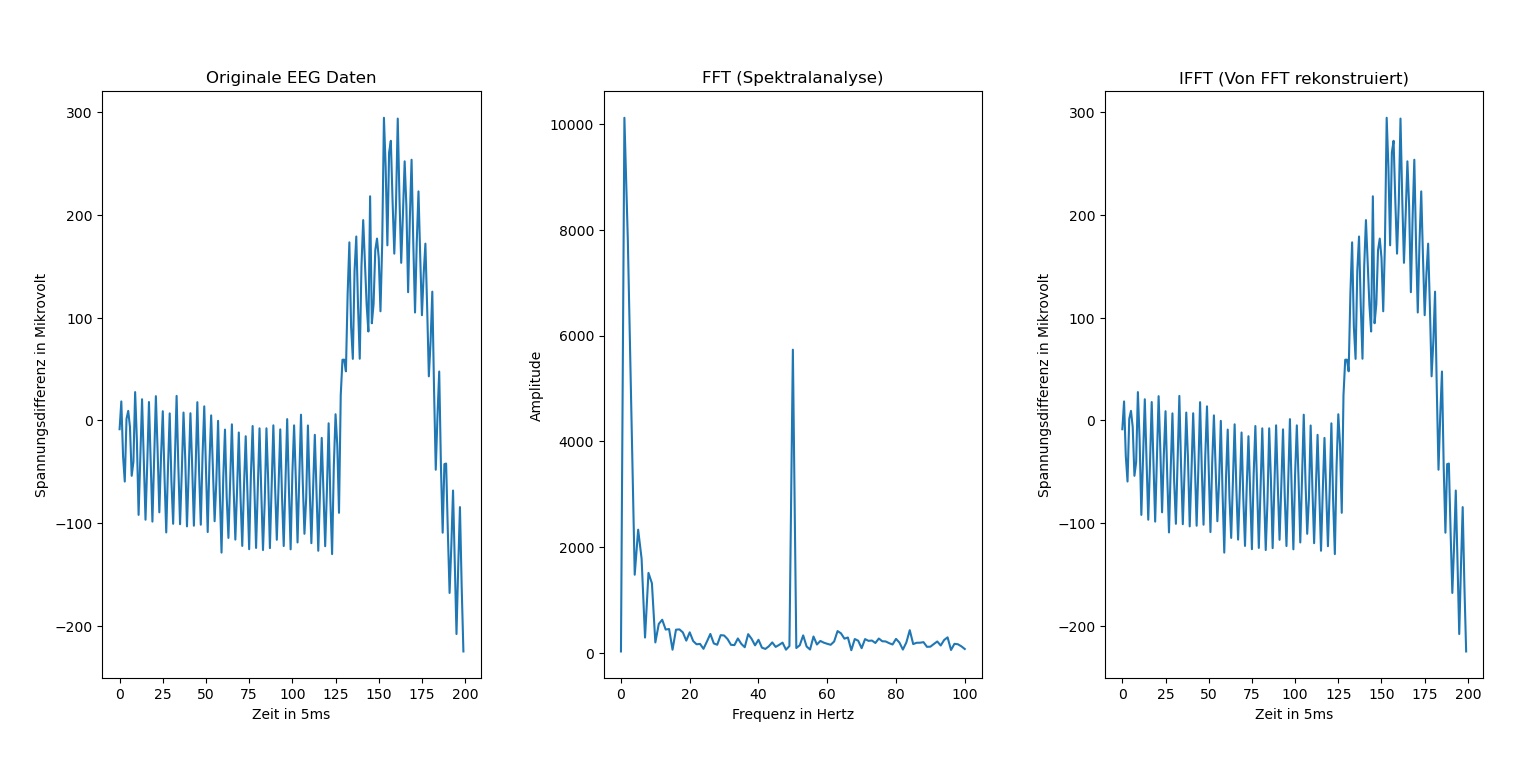
\includegraphics[width=\textwidth]{pictures/blink_fft_ifft.png}
		\caption{Das EMG-Signal eines Blinzelns, die Amplituden des FFT dieses Signales, und eine Rekonstruktion des Signals durch IFFT}
		\label{EEG-IFFT}
	\end{figure}

	Vor der Implementation von FFT haben wir zuerst getestet, ob eine Spektralanalyse für unseren Zweck überhaupt sinnvoll wäre. Dazu haben wir die Ergebnisse der FFT von Elektroenzephalogrammen mit Blinzeln und ohne Blinzeln verglichen. Wie man in Abbildung \ref{EEG-FFT} sehen kann, gibt es vor allem im niedrigeren Frequenzbereich einen klaren Unterschied.
	Die KI sollte in der Lage sein, diesen Unterschied zu erkennen. Eine FFT wäre also zur Vorverarbeitung der Daten geeignet.

	%\begin{figure}[H]
	%	\fig{
	%	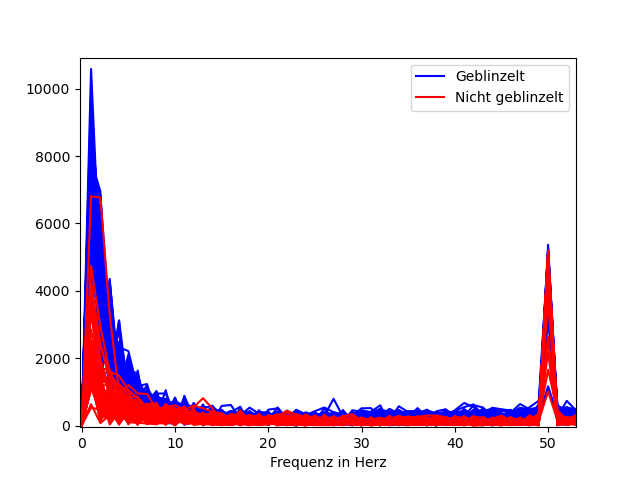
\includegraphics[width=0.9\textwidth]{pictures/Die_FFTs_der_EMG-Daten.png}
	%	\caption{Die FFT unserer EEG-Daten}
	%	\label{EMG-FFT}}
	%\end{figure}

	\begin{figure}[H]
		\fig{
		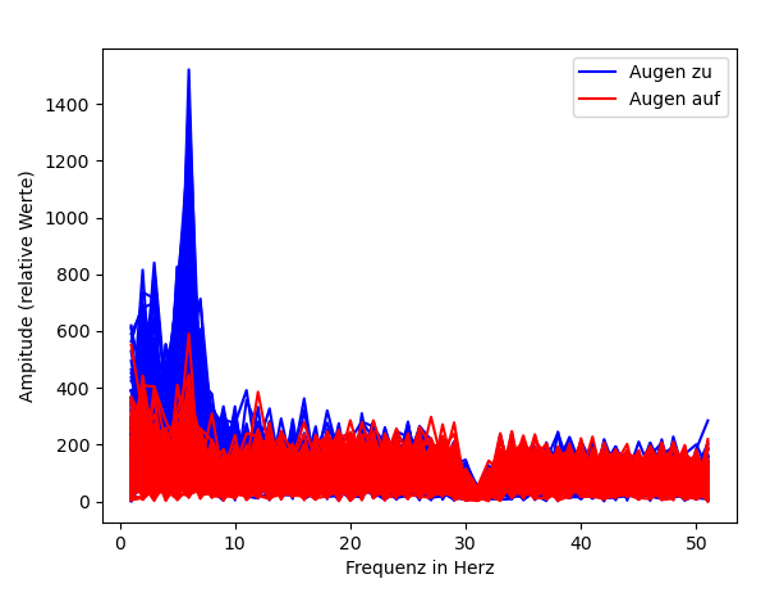
\includegraphics[width=0.9\textwidth]{pictures/Die_FFTs_der_EEG-Daten.png}
		\caption{Die Amplituden für die Frequenzen 1-50 Hertz von unseren Trainings- und Testdaten (EEG, Konfiguration 2), berechnet durch die FFT. Jede Linie entspricht einem Datensatz. 
		Blaue Linien: durchgehend geschlossene Augen, rote Linien: geöffnete Augen.}
		%Bei den blauen wurde geblinzelt, bei den roten nicht.}
		\label{EEG-FFT}}
	\end{figure}
	
	Ob die FFT Analyse einen großen Vorteil zu den Rohdaten darstellen wird, werden wir in den Ergebnissen sehen müssen, jedoch liegt es nahe, da die KI sich auf einige wenige, wichtige Inputs konzentrieren kann. Denn wie man sehen kann, ist der Unterschied in den höheren Frequenzbereichen nicht so groß und vermutlich für eine sichere Erkennung nicht unbedingt notwendig.

	Die FFT ist außerdem sehr schnell, auf unserem Test-System braucht sie für die Verarbeitung von einer Sekunde Messdaten von zwei Elektroden im Schnitt \qty{22}{\micro\second}. Ein weiterer Vorteil der FFT ist, dass wir weniger Inputs haben. Wir brauchen allerhöchstens die Amplituden für 1-100 Hertz, alles darüber hinaus kann unser EEG sowieso nicht akkurat wahrnehmen. Mit 100 Inputs (die Frequenzen) statt 200 Inputs (jede einzelne Spannungsdifferenz) kann unsere KI schneller lernen und schneller eine Erkennung durchführen.

	Dennoch wollen wir das Programm auch ohne FFT ausprobieren -- wenn die Ergebnisse gleich gut sind, würde es sich trotzdem lohnen, auf FFT zu verzichten, da für FFT auch die Installation eines weiteren Packages (FFTW) notwendig ist. 

	\subsubsection{Neuronales Netz}

	Ein neuronales Netzwerk besteht aus drei Teilen: dem Input Layer, den Hidden Layers und dem Output Layer. 
	Der Input Layer ist eine Liste aus Zahlen zwischen 0 und 1. Er gibt an, welche Eingaben (Inputs) das Netzwerk bekommen soll, z. B. die Grauwerte der Pixel eines Bildes.
	Die Hidden Layers sind eine Ansammlung von in mehrere Layer (Schichten) unterteilten Neuronen.
	Jedes Neuron besitzt eine Aktivierung (Activation), die als Zahl zwischen 0 und 1 angegeben werden kann, und einen Bias (Verzerrung), der eine beliebige Zahl sein kann. Die Neuronen verschiedener Layer sind alle durch sogenannte Gewichte (Weights) verbunden, die ebenfalls einen beliebigen Wert haben können.
	Die Outputs sind dann lediglich die Aktivierungen der Neuronen im Output Layer.

	\threesub{Forward Pass}

	Zur Berechnung der Aktivierung der Neuronen gibt es den sogenannten Forward Pass. Dabei beginnt man im ersten Hidden Layer damit, für alle Neuronen den sogenannten Netzinput (auch net input) zu berechnen. Um den Netzinput eines Neurons zu berechnen, werden alle Aktivierungen des vorherigen Layers mit den von dem Neuron dorthin führenden Gewichten multipliziert und aufsummiert. Der Bias ist eigentlich auch ein Gewicht, jedoch ist er mit einem Neuron verbunden, das immer die Aktivierung 1 hat.

	\begin{wrapfigure}{r}{0.4\textwidth}
		\centering
		\vspace*{-5mm}
		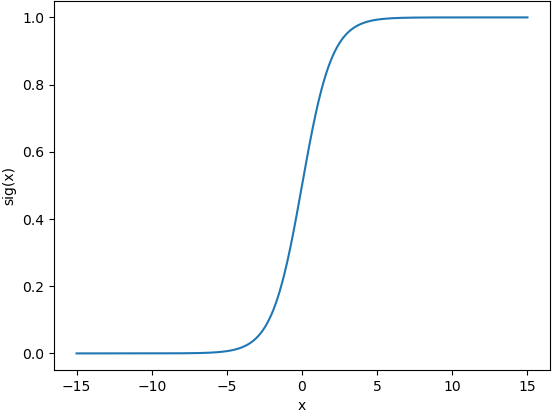
\includegraphics[width=0.4\textwidth]{pictures/sig_func.png}
		\caption{Graph der Sigmoidfunktion. Wir nutzen die Sigmoidfunktion um die Aktivierung, $sig(x)$, aus dem Netzinput, $x$, zu berechnen.}
		\label{sig_func}
	\end{wrapfigure}

	Um aus diesem Netzinput nun die Aktivierung zu berechnen, benötigt man eine Aktivierungsfunktion, die dafür sorgt, dass die Aktivierung immer zwischen 0 und 1 liegt. Wir haben dafür eine Sigmoidfunktion benutzt, die eine Zahl nimmt und einen Wert zwischen 0 und 1 ausgibt (siehe Abbildung \ref{sig_func}). Dies wird dann für jedes Neuron in jedem Layer wiederholt. Da man aber immer die Aktivierungen des vorherigen Layers benötigt, muss man das ganze vom Input Layer zum Output Layer durchführen. Daher auch der Name Forward Pass. Die Interpretation der Outputs hängt von den Trainingsdaten ab.
	
	Die allgemeine Formel für die Aktivierung eines Neurons lautet also:


	\form{
	\[
		\sig(x)=\frac{1}{1+e^{-x}}
		\]
	\[
		a_{j} = \sig\left(\sum_{L} (a_{L} * W_{Lj}) + b_{j}\right)
		\]}
	
	\noindent wobei $a_j$ die Aktivierung des Neurons $j$, $L$ der vorherige Layer, $a_L$ der Vektor aller Aktivierungen des Layers $L$, $W_{Lj}$ der Vektor aller Gewichte zwischen dem Neuron $j$ und den Neuronen des Layers $L$, und $b_j$ der Bias des Neurons $j$ ist. \cite{brotcrunsher:forwardpass}	
	
	\threesub{Loss/Cost} 

	Um zu bestimmen, wie gut ein bestimmtes neuronales Netz ist, gibt es die sogenannte Cost-Funktion (auch Loss-Funktion genannt), die mithilfe von Trainingsdaten funktioniert.
	Trainingsdaten bestehen aus einer Liste aus Trainingsdatensätzen. Jeder dieser Datensätze beinhaltet Inputs für das Netzwerk und die richtigen Outputs dafür. Machine Learning, das mit solchen Trainingsdaten arbeitet, wird Supervised Learning genannt.

	Die Funktion für die Cost des Output-Layers und somit des gesamten Netzwerkes (für einen Trainingsdatensatz) lautet wie folgt:

	\form{ \[
		C_0 = (a_L - y)^2
	\]}

	%C0 = (aL − y)2 

	\noindent wobei $C_0$ die Cost des Output-Layers, $L$ der letzte Layer (Output Layer), $a_L$ der Vektor aller Aktivierungen des Layers $L$, und $y$ ein Vektor der richtigen Outputs für die Inputs, mit denen die Aktivierungen berechnet wurden, ist. 
	
	Um die Cost zu berechnen, muss man also für alle Output Neuronen die Differenz der gegebenen und der richtigen Aktivierungen bilden. Danach muss man diese Differenzen quadrieren und am Ende alle Ergebnisse aufsummieren. Dies kann man für alle Trainingsdatensätze wiederholen und von allen Costs den Durchschnitt nehmen, um die allgemeine Performance eines Netzwerkes zu überprüfen. Diese Art der Cost-Funktion wird mittlere quadratische Abweichung (mean squared error, kurz MSE) genannt. 
	
	Zusammenfassend kann man also sagen, dass die Cost die Abweichung von den berechneten und den richtigen Outputs angibt. Aufgrund des Trainingsdatensatzes weiß man nun, wie der Output Layer verändert werden
	muss.

	\threesub{Backpropagation}

	Doch wie verändert man nun die Aktivierungen des Output-Layers? Es müssen alle Gewichte und Biases davor angepasst werden. Um nun zu wissen, wie ein Gewicht verändert werden muss, gibt es folgende Funktion:

	\form{\[
		\Delta W_{ij} = \epsilon * \delta_i * a_j
	\]}
%
	Hier ist  $\Delta W_{ij}$ der Wert, um den das Gewicht $W$ zwischen den Neuronen $j$ und $i$ verändert werden muss, $\epsilon$ die Lernrate (meist ein kleiner Wert wie 0.001), $\delta_i$ eine Annäherung der Ableitung der Cost des Neurons $i$ im Verhältnis zum Gewicht $W_{ij}$, und $a_j$ die Aktivierung des Neurons $j$. Was dabei oft verwirrend ist: $j$ bezeichnet das Neuron, welches zuerst kommt, und $i$ das Neuron, welches danach kommt (Reihenfolge im Forward-Pass), obwohl es bei $W_{ij}$ andersherum steht.

	Für den Bias wird die gleiche Formel benutzt, mit der Ausnahme, dass $a_j$ immer 1 ist und so wegfällt. Der Grund dafür liegt darin, dass der Bias, wie in der Struktur beschrieben, eigentlich nur ein Gewicht ist, das mit einem Neuron verbunden ist, welches immer eine Aktivierung von eins hat.

	Um nun $\delta_i$ für den Output Layer zu berechnen, gibt es folgende Gleichung: 

	\form{\[
		%\delta_i = \sig '\left({\netin}_i\right) * (a_i (\textrm{soll}) - a_i (\textrm{ist})) 
		\delta_i = \sig '\left(x_i\right) * (a_i (\textrm{soll}) - a_i (\textrm{ist})) 
	\]}
%
	wobei $\sig '(x)$ die Ableitung von $\sig(x)$ ist, also $\sig'(x) = \sig(x) * (1 - \sig(x))$, $x_i$ der Netzinput des Neurons $i$, $a_i(\textrm{soll})$ die Aktivierung, die das Neuron haben sollte (also das gleiche wie $y$), und $a_i(\textrm{ist})$ die Aktivierung, die das Neuron hat.
%
	Mit dieser Formel wird berechnet, welche Aktivierung das Neuron haben sollte, was an $a_i(\textrm{soll}) - a_i(\textrm{ist})$ erkennbar ist. Die Aktivierungsfunktion mit dem Netzinput wird als Faktor mit einberechnet, da möglichst nur die Gewichte stark verändert werden sollen, die bei dem Trainingsdatensatz eine hohe Aktivierung haben, also durch diese Inputs besonders angesprochen werden. So werden zum Beispiel beim Sortieren nur die Neuronen stark miteinander verknüpft, die für ein bestimmtes Muster verantwortlich sind.
	
	Für die Neuronen der Hidden Layers muss man alle $\delta$'s des nächsten Layers mit den von dem Neuron dorthin führenden Gewichten multiplizieren und dann summieren. Dadurch werden die Änderungen, die die Aktivierungen dieser Neuronen brauchen ($\delta$), zusammengerechnet, da natürlich die Aktivierungen im nächsten Layer unterschiedliche Änderungen in dem gleichen Neuron benötigen.
	
	Durch die Multiplikation mit den dahin führenden Gewichten werden diese Änderungen gewichtet, da sie auf einige Neuronen größere Auswirkungen haben als auf andere. Wie beim Output Layer auch wird diese Summe noch mit $\sig'(x)$ multipliziert, um die Aktivierung durch bestimmte Muster angesprochener Neuronen noch weiter zu erhöhen und weniger/kaum angesprochener Neuronen zu senken, sodass die Ergebnisse besser und eindeutiger werden. Die Formel hierfür lautet:

	\form{\[\sig'(x_i) * \sum_{L}{\left(\delta_L\ast W_{Li}\right)}\]}
%
	\noindent wobei $L$ der nächste Layer, $\delta_L$ der Vektor aller $\delta$'s des Layers $L$, und $W_{Li}$ der Vektor aller Gewichte, die ein Neuron des nächsten Layers und Neuron $i$ verbinden, ist.
%
	Da immer der (im Forward Pass gesehene) nächste Layer benötigt wird, ergibt es Sinn, diese Optimierung beim Output Layer zu starten und dann rückwärts die \mbox{$\delta$-Werte} für jeden Layer zu berechnen und für die nächsten Berechnungen zu speichern -- daher auch der Name Backpropagation. \cite{MITNeuronale} \cite{3b1b:nn} \cite{brotcrunsher:backwardpass}

	\threesub{Flux}

	Wir haben in unserem letzten Projekt bereits ein neuronales Netzwerk mit dieser Funktionsweise selbst programmiert, um es besser verstehen zu können. \cite{AIComposer} Für dieses Projekt haben wir allerdings das Package Flux benutzt, welches die gleichen oder bessere Ergebnisse liefern sollte, mit deutlich besserer Performance, da es stark optimiert und sehr viel weiter entwickelt wurde. \cite{Flux.jl-2018}

	\subsubsection{Roboter}

	Für unseren Roboter haben wir uns entschieden, Lego Mindstorms EV3 Motoren zu benutzen, die von einem EV3-Brick gesteuert werden, der wiederum von einem Raspberry Pi 3B+ gesteuert wird (siehe Abbildungen \ref{robot-funktion} und \ref{Robot}). Der Grund dafür, dass wir keine Motoren direkt mit dem Raspberry Pi steuern, ist, dass wir schon alle Teile für einen EV3 Roboter haben. Somit müssten wir entweder neue Motoren kaufen oder passende Adapter finden, welche meist nur mit der Sprache C und Python funktionieren und teuer sind.

	Der Roboter, zu sehen in Abbildung \ref{Robot}, wurde von Alexander Reimer, Ino Saathoff, und Oliver Samkovskij im Rahmen der Robotik-AG unserer Schule für den RoboCup entwickelt. Die Steuerung in Julia wurde jedoch von uns selbst programmiert. Danke an Ino und Oliver, dass ihr uns erlaubt, den Roboter auch hierfür zu nutzen!

	\begin{figure}[H]
		\centering
		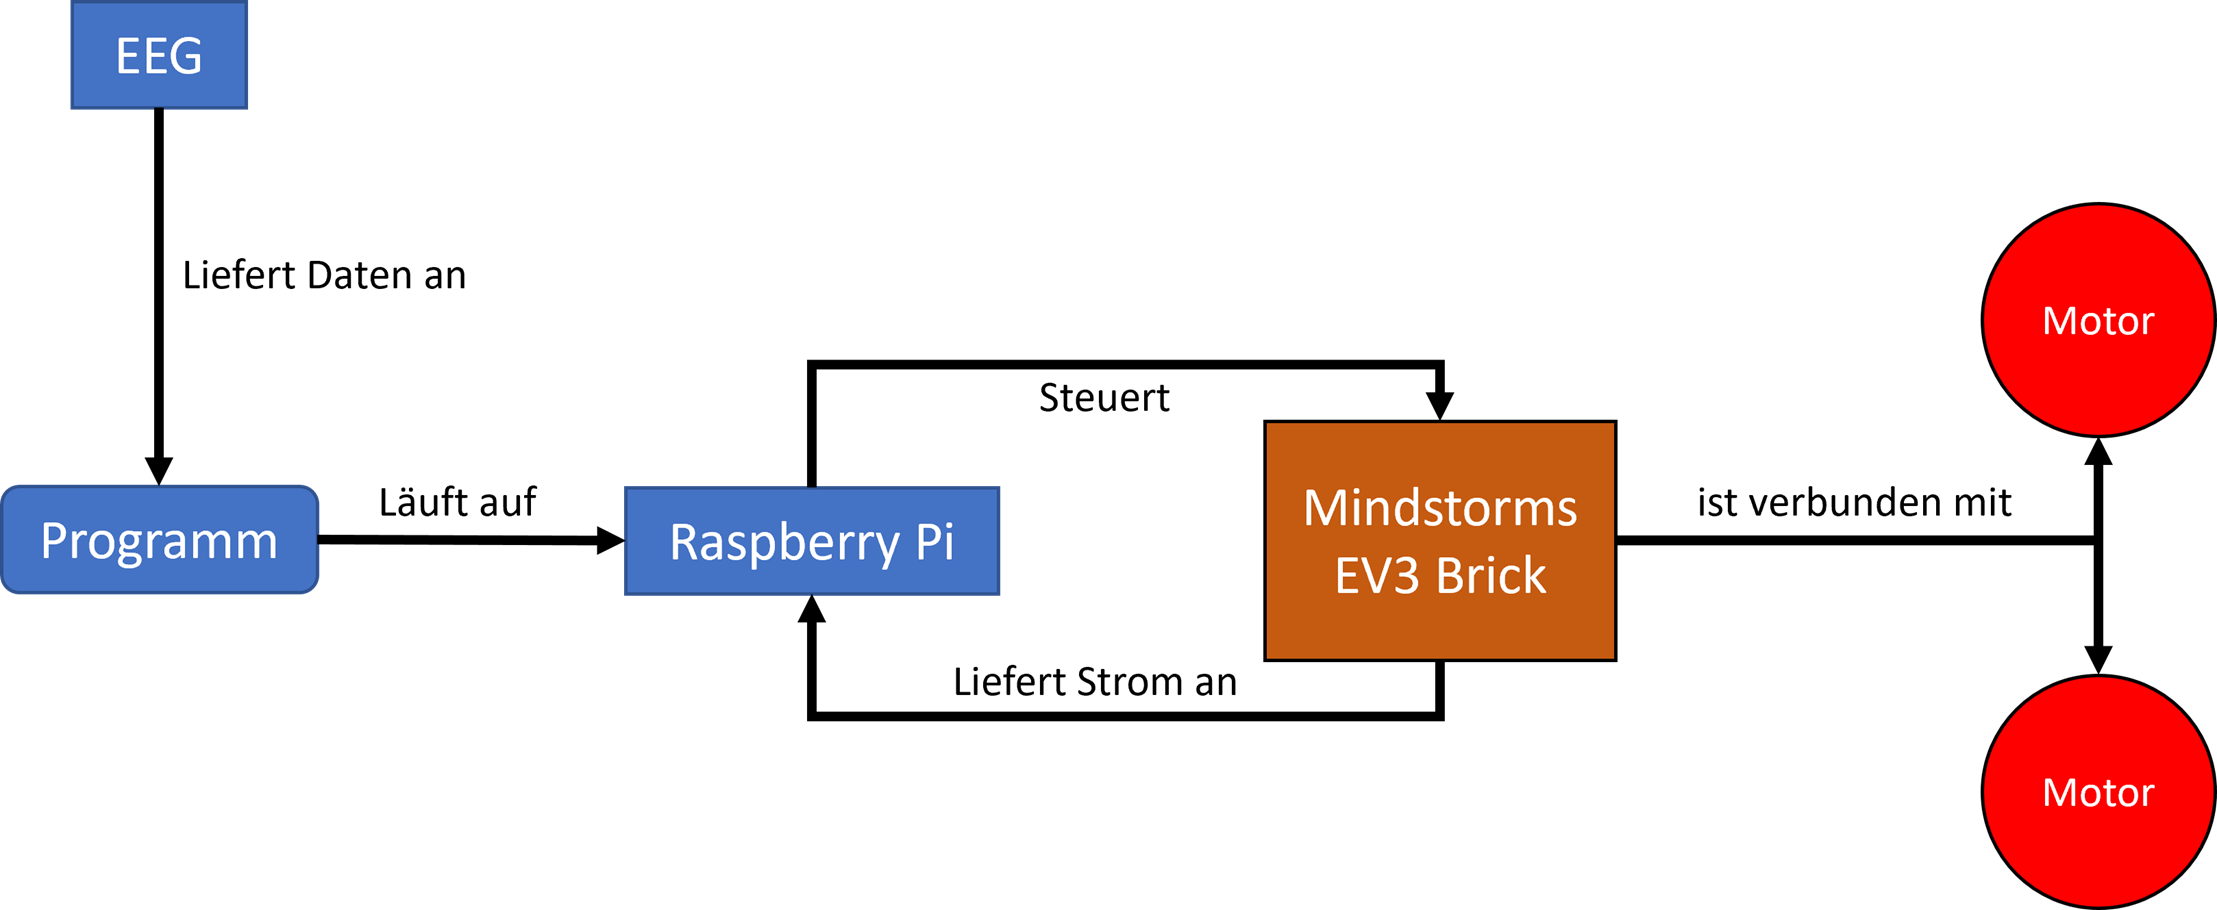
\includegraphics[width=0.8\textwidth]{pictures/roboter-funktionsweise.png}
		\caption{Darstellung des Informationsflusses in unserem Experiment. Die über das EEG aufgenommen Gehirnaktivitäten werden durch das neuronale Netz analysiert. Das Ergebnis wird an den Raspberry Pi weitergeleitet, welcher mittels des EV3-Bricks die Motoren ansteuert.}
		\label{robot-funktion}
	\end{figure}

	\begin{figure}[H]
		\centering
		\includegraphics[width=0.5\textwidth]{pictures/roboter-annotated.png}
		\caption{Unser Roboter (ohne Raspberry Pi, der über dem EV3-Brick angebracht ist). Die extra mittleren Motoren, die Konstruktion vorne, sowie die Sensoren vorne und unten sind für unser Projekt nicht relevant.}
		\label{Robot}
	\end{figure}

	Die Steuerung besteht aus zwei Komponenten: dem Brick und dem Computer.
	%
	Auf dem EV3-Brick wurde mit einer SD-Karte das Betriebssystem ev3dev installiert. Dieses gibt neben komplettem Zugriff auf das Debian-Betriebssystem des Bricks auch Zugriff auf die Motoren. Ev3dev übernimmt die tiefgreifende, direkte Kontrolle der Motoren, und ermöglicht eine Steuerung / einen Informationsabruf über verschiedene Dateien im \filepath{/sys/class} Verzeichnis (s. Beispiele in Tabelle \ref{beispiel-dateien})

	\begin{table}[H]
		{\centering
		\begin{tabular}{p{0.5\textwidth}p{0.45\textwidth}}
			\toprule
			Dateipfad & Funktion \\
			\midrule
			\filepath{/sys/class/tacho-motor/motor<x>/address} & Der Port, an dem der Motor angeschlossen ist (outA, outB, etc.) \\
			\filepath{/sys/class/tacho-motor/motor<x>/command} & Einen \enquote{Befehl} an den Motor senden, wie z.B. \cmd{stop}, \cmd{run-timed} oder \cmd{run-forever} \\
			\filepath{/sys/class/tacho-motor/motor<x>/commands} & Alle verfügbaren Befehle. \\
			\filepath{/sys/class/tacho-motor/motor<x>/speed\_sp}, \path{/sys/class/tacho-motor/motor<x>/duty_cycle_sp} & Die aktuelle Geschwindigkeit des Motors auslesen oder setzen.\\ 
			... & ...\\
			\bottomrule
		\end{tabular}
		\caption{Einige Beispieldateien für die Steuerung eines Motors auf ev3dev. \filepath{<x>} ist die Nummer des Motors. Mehr Informationen dazu gibt es in der Dokumentation von ev3dev. \cite{ev3dev-docs}}
		\label{beispiel-dateien}}
	\end{table}

	Auf dem Computer (ein Raspberry Pi 3B+) verwenden wir SSHFS, um einen Mount zu erstellen, mithilfe dessen wir über USB vom Pi aus auf diese Dateien zugreifen können.
%
	In einer von uns eigens entwickelten Julia-API haben wir dann Funktionen implementiert, welche dem Nutzer ein unkompliziertes Steuern des Roboters erlaubt. Dabei machen die low-level Funktionen nichts anderes, als z.B. die vom Nutzer gewünschte Geschwindigkeit in die entsprechende Datei zu schreiben.
%
	Den Code dazu haben wir auf GitHub veröffentlicht, unter dem Namen ev3dev.jl. \cite{ev3dev}

	Das Programm sollte ebenfalls mit dem Raspberry Pi 4B funktionieren, jedoch haben wir momentan nur einen Raspberry Pi 3B+. Dieser ist vergleichsweise sehr schwach, mit nur 1\,GB Arbeitsspeicher. Vor allem die Menge an Arbeitsspeicher stellt ein Problem dar, da sie nicht groß genug ist, um überhaupt alle benötigten Packages zu laden.
%
	Deshalb müssen wir jetzt erstmal einen Umweg gehen: Anstatt das ganze Programm direkt auf dem Raspberry Pi am Roboter auszuführen, erstellen wir mit SSHFS auf unserem Laptop einen Mountpoint, welcher über WLAN auf den Mountpoint auf dem Raspberry zugreift, und so über diesen Zugriff auf das \filepath{/sys/class}-Verzeichnis des Bricks hat. Die Auslesung der EEG-Daten, das Auswerten durch das neuronale Netzwerk, und die Steuerung der Motoren können so alle auf dem Laptop stattfinden.
	

	\subsubsection{Übersicht des Ablaufs unseres Programmes in einem Diagramm}
	\begin{figure}[H]
		\fig{
		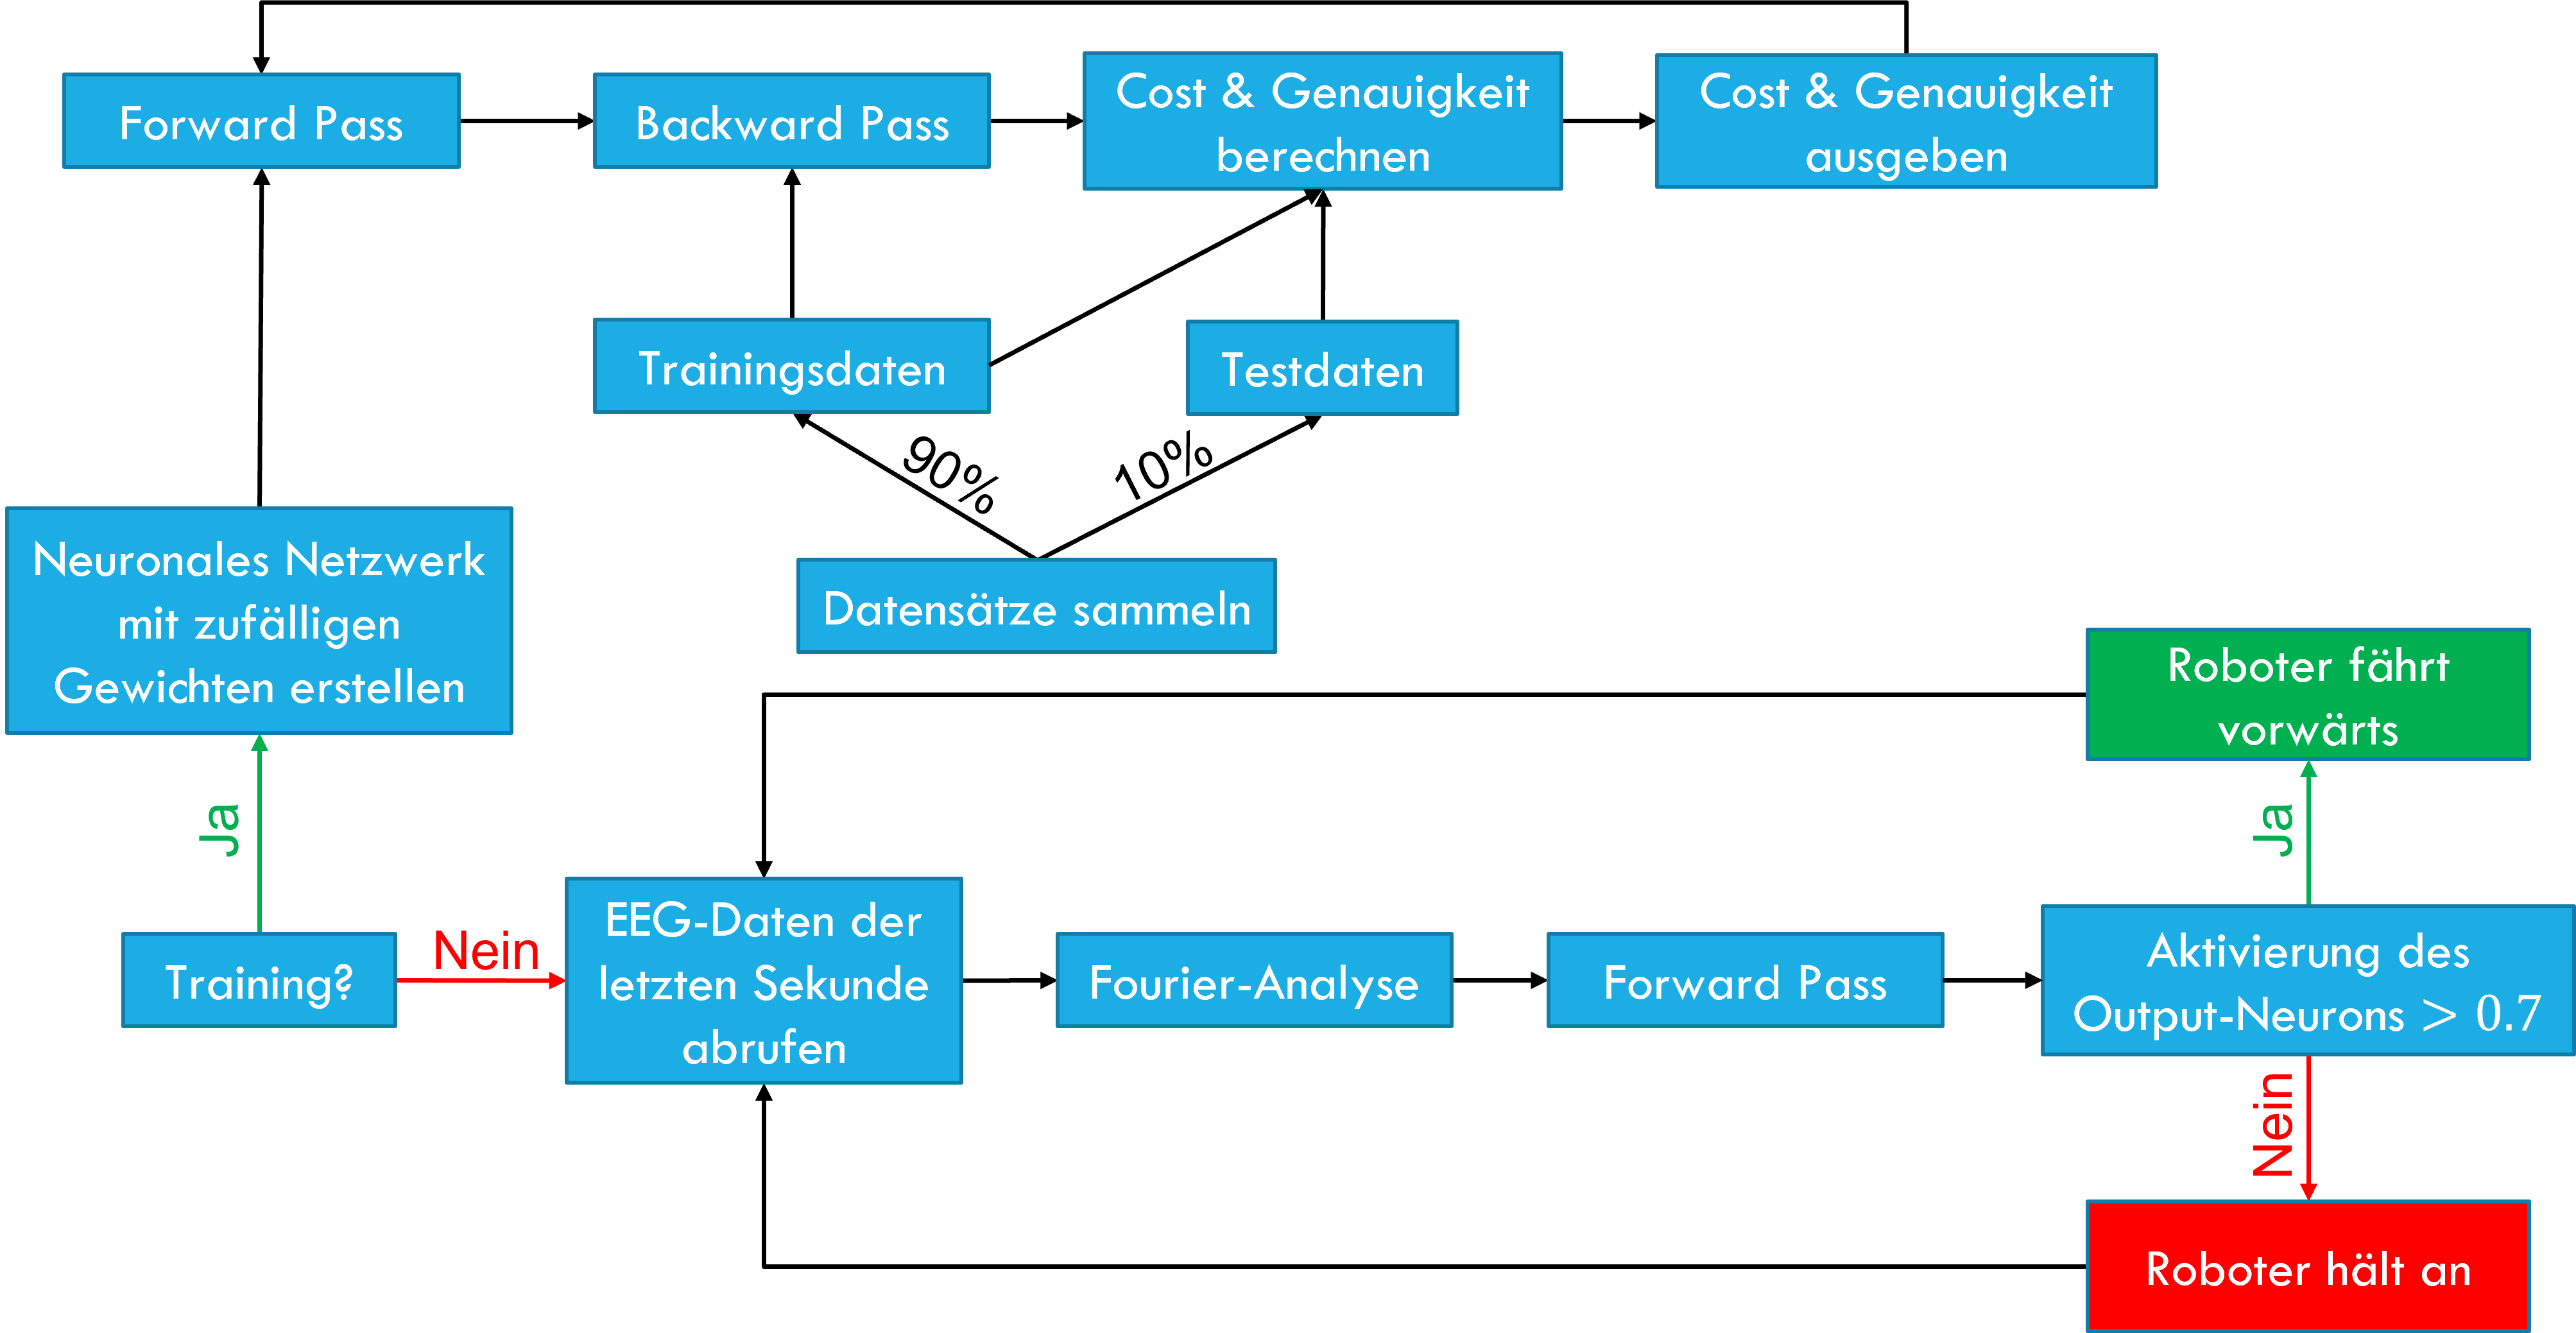
\includegraphics[width=\textwidth]{pictures/programm-ablauf.png}
		\caption{Eine Übersicht des Ablaufs unseres Programmes in einem Diagramm. Wenn wir trainieren, dann erstellen wir zuerst ein neuronales Netzwerk mit zufälligen Gewichten. Danach trainieren wir es mithilfe der Trainingsdaten, die 90\% unserer vorher gesammelten Datensätze sind. Mit den restlichen 10\%, die die Testdaten formen, sowie den Trainingsdaten, berechnen wir die aktuelle Genauigkeit und Cost. Dies wird wiederholt, bis eine zufriedenstellende Leistung erreicht wurde. Wenn wir das Programm nutzen, also nicht trainieren wollen, dann rufen wir durchgehend die EEG-Daten der letzten Sekunde ab, berechnen die Amplituden der Frequenzen mit FFT, und geben diese an das neuronale Netz als Inputs. Falls die Aktivierung des Output-Neurons über dem Schwellenwert liegt, dann fährt der Roboter vorwärts, und falls sie darunter liegt, hält der Roboter an. Den Schwellenwert für die Aktivierung des Output-Neurons haben wir durch Beobachtung des Wertes in Tests sowie Ausprobieren bestimmt.}
		\label{programm-ablauf}}
	\end{figure}

	%\begin{figure}[H]
	%	\centering
	%	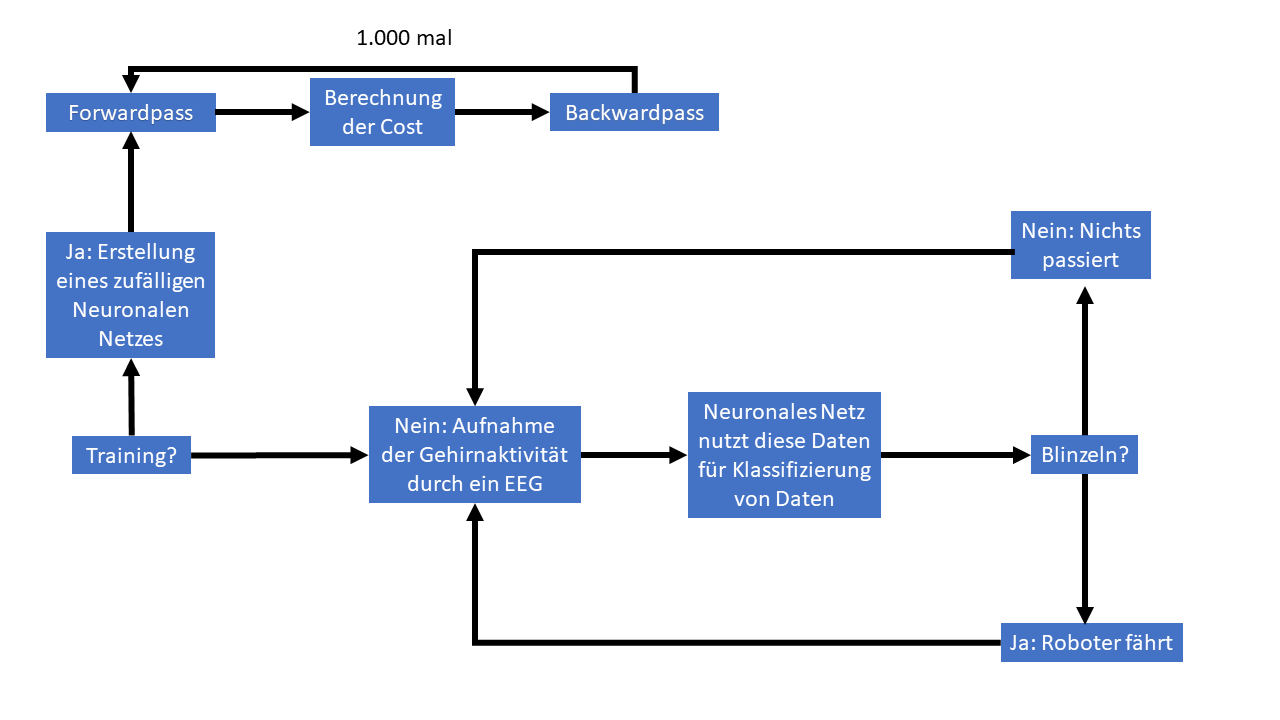
\includegraphics[width=0.9\textwidth]{pictures/Abbildung-des-Programms.png}
	%	\caption{Funktionsweise des Programms}
	%	\label{Gesamtfunktion}
	%\end{figure}

	%\newpage
	%\subsection{Funktionsweise des Programms}

	%\begin{figure}[h!]
	%	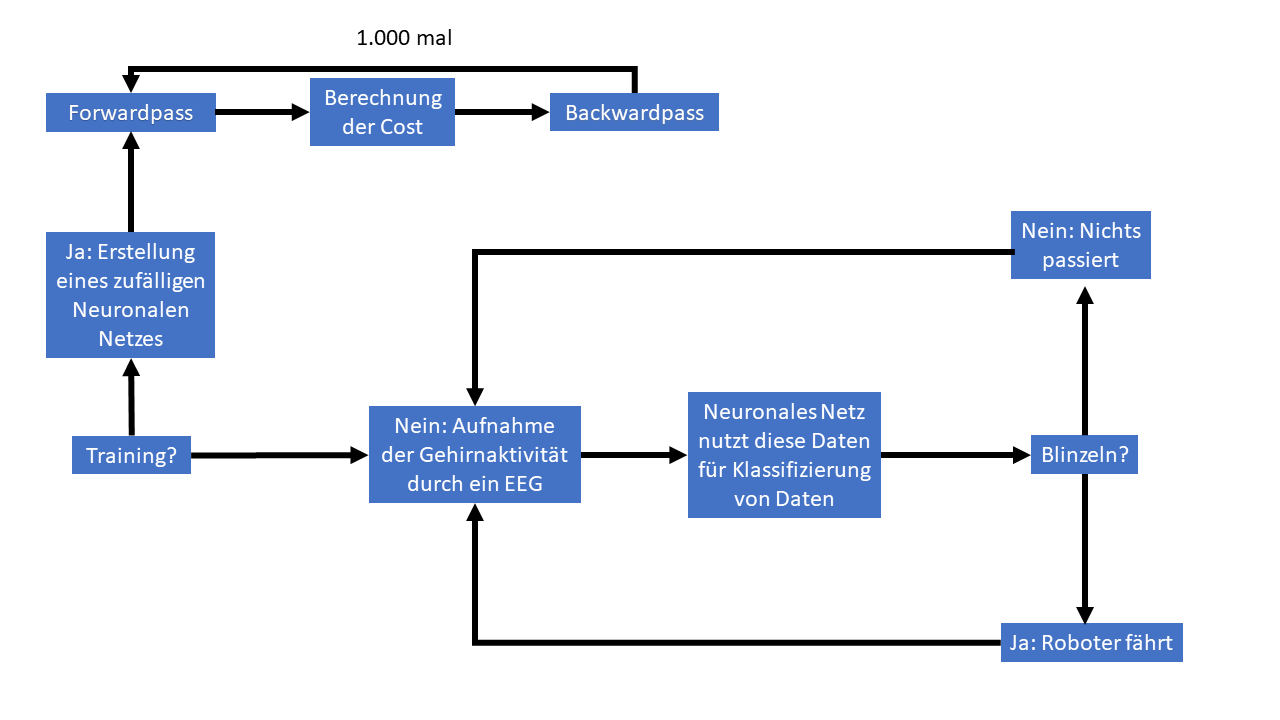
\includegraphics[width=\textwidth]{pictures/Abbildung-des-Programms.png}
	%	\caption{Funktionsweise des Programms}
	%\end{figure}

	\section{Ergebnisse}

	Beim Erkennen von Blinzeln mit EMG (Konfiguration 1) erhielten wir, sowohl mit als auch ohne FFT, eine Testdaten-Genauigkeit von 95\% (siehe Abbildung \ref{training-emg}), in einigen undokumentierten Durchläufen auch 100\%. Mit der Genauigkeit ist gemeint, welchen Anteil der gegebenen Datensätze das neuronale Netzwerk korrekt klassifizieren konnte. Dabei ist vor allem die Testdaten-Genauigkeit relevant, da diese die Genauigkeit mit den Testdaten angibt. Die Testdaten sind nicht in den Trainingsdaten enthalten, sodass das neuronale Netzwerk nicht mit ihnen trainiert wurde und so mit ihnen komplett neue, unbekannte Fälle simuliert werden können.

	\begin{figure}[H]
		\fig{
		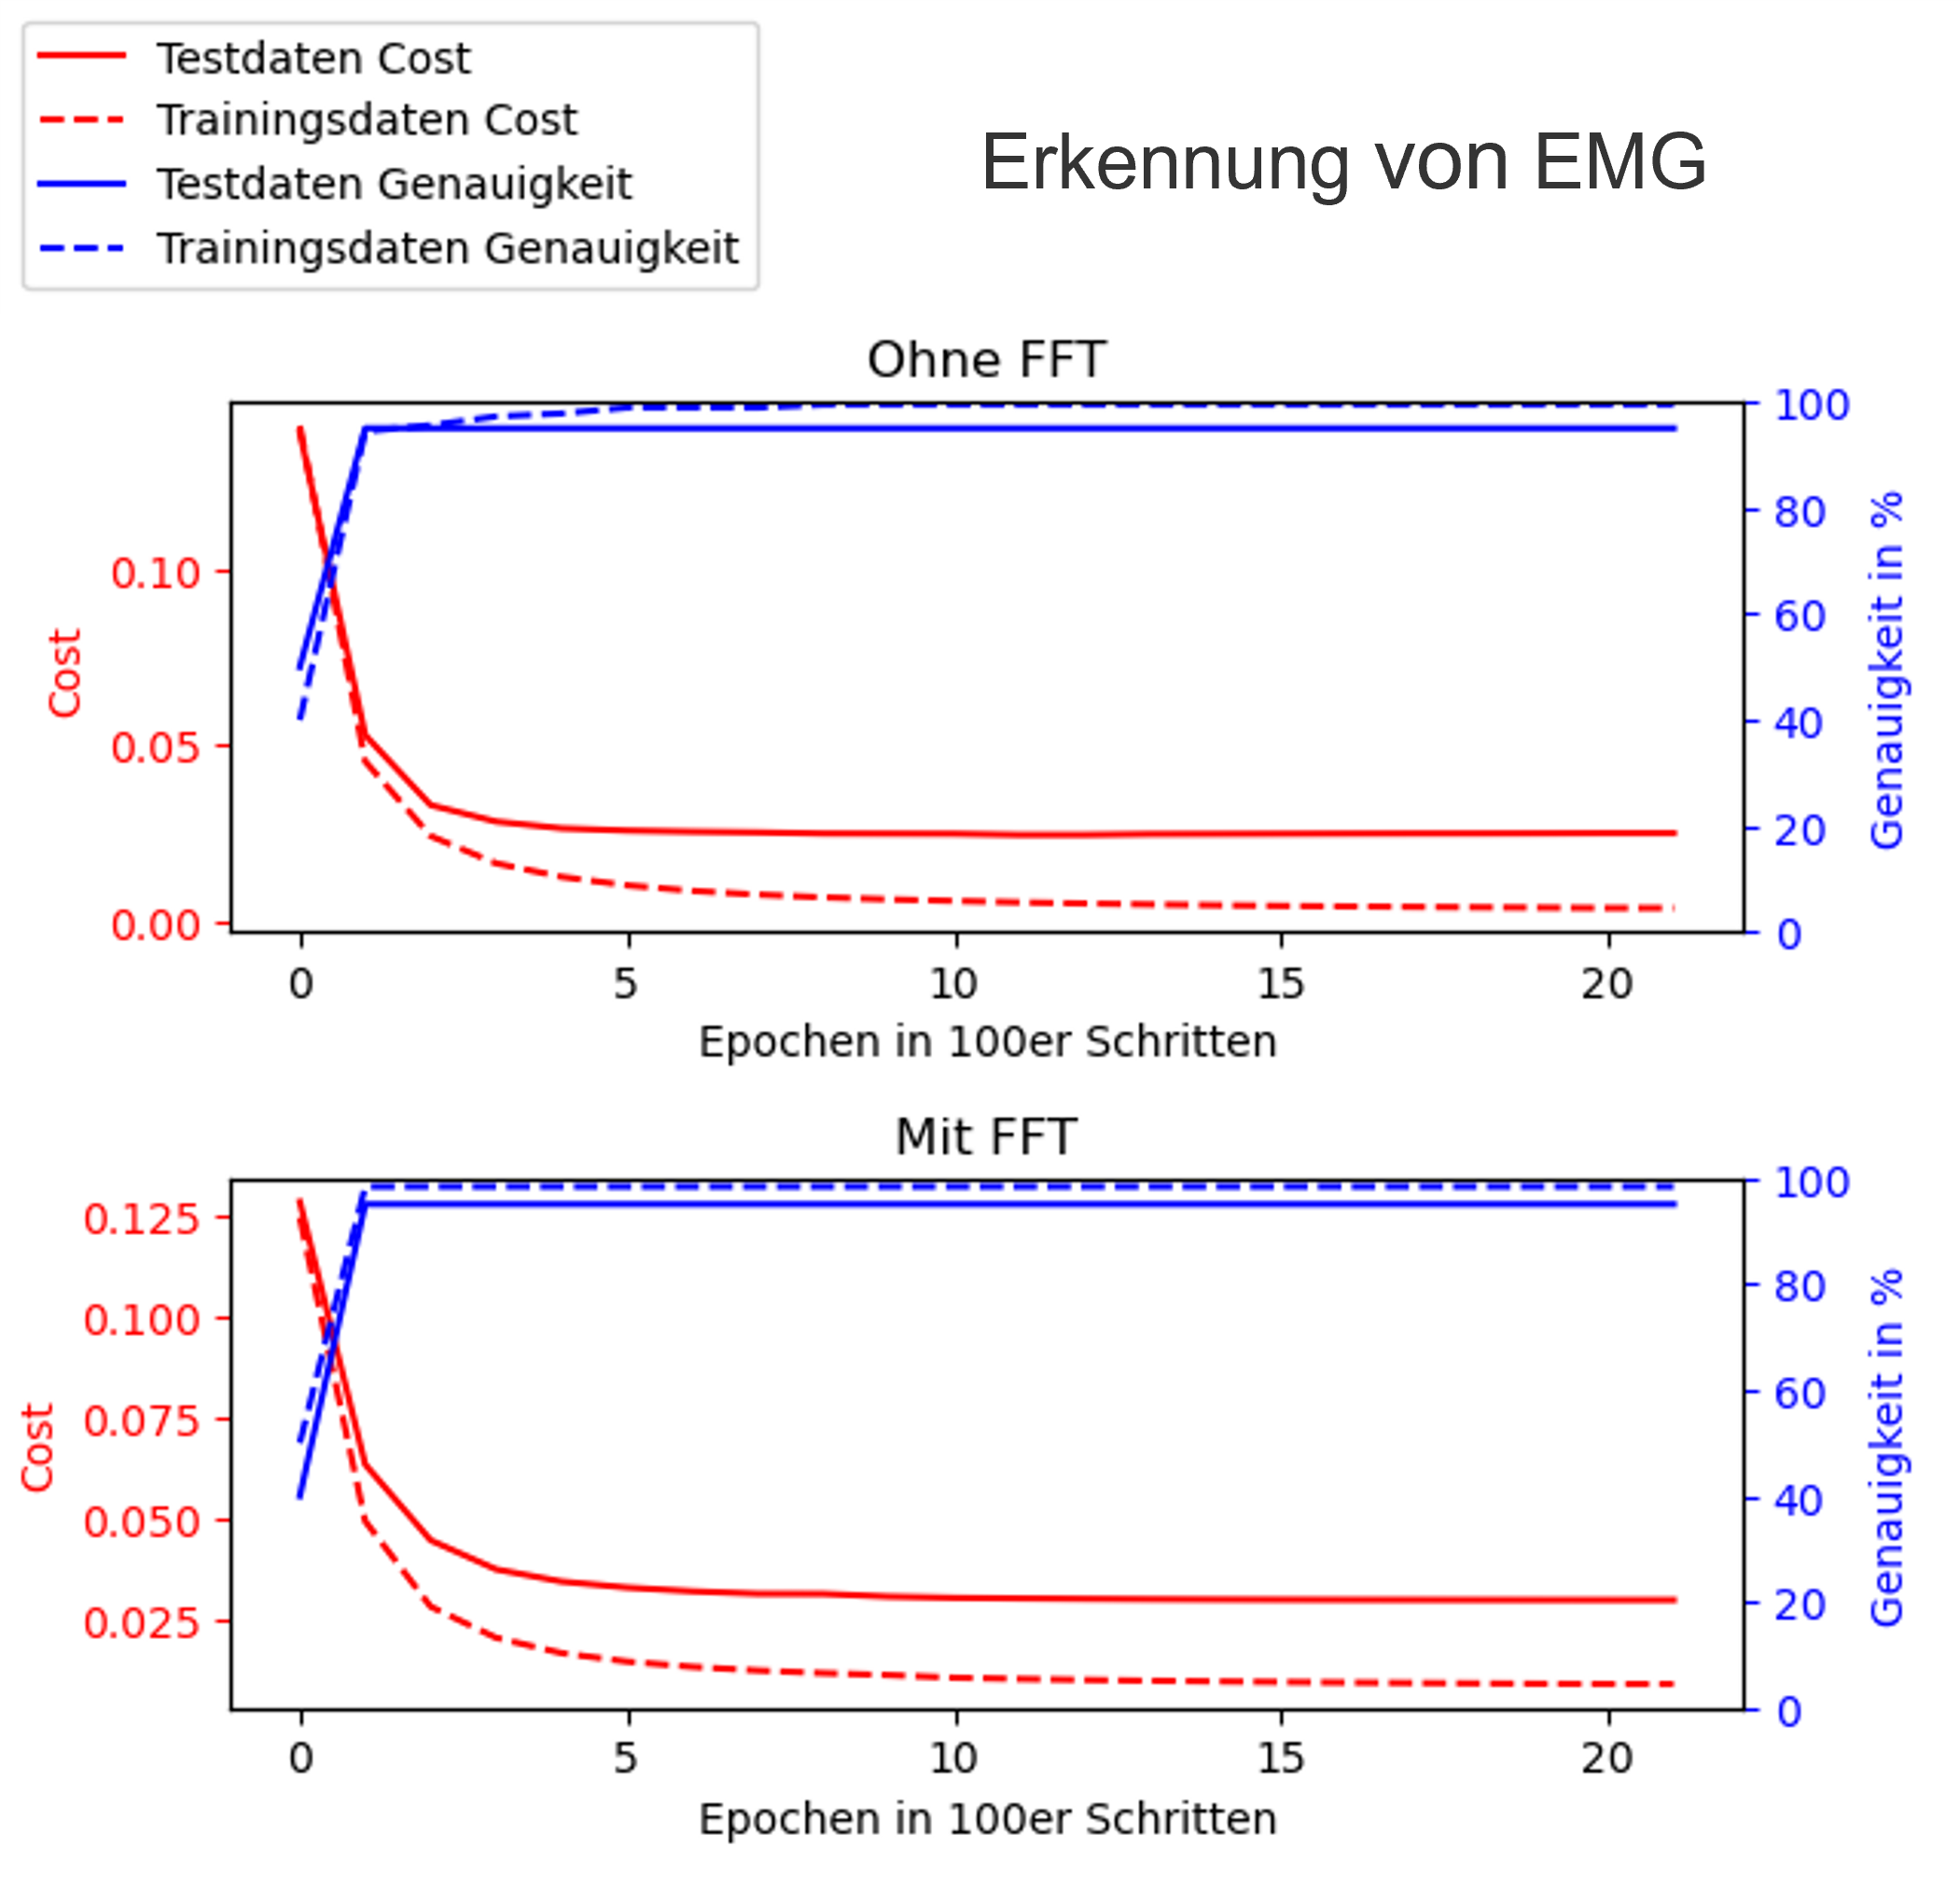
\includegraphics[width=0.7\textwidth]{pictures/Trainingsprozess_EMG_FFT_vs_kein_FFT2.png}
		\caption{Es wurde EMG benutzt. Zu sehen ist der Cost- und Genauigkeitsverlauf der Test- und Trainingsdaten beim Trainieren des Netwerkes, oben ohne Vorverarbeitung durch FFT und unten mit. Eine Epoche entspricht jeweils einer Backpropagation mit allen Trainings-Datensätzen.}
		\label{training-emg}}
	\end{figure}

	
	Wir hatten jeweils 100 Trainingsdatensätze für die Fälle, dass geblinzelt und nicht geblinzelt wurde.
	Für die Struktur der Hidden Layers des Netzwerkes haben wir uns entschieden, da wir einige ausprobiert haben und diese konsistent gute Ergebnisse (90-100\% Testdaten-Genauigkeit) mit kurzen Trainingszeiten (ca. 3 Minuten für 1000 Epochen, mit FFT) geliefert haben. Sie ist zu sehen in Abbildung \ref{emg-netzstruktur}.
		Auch ein realer Test mit einer Testperson lief gut, wie man in der Aufnahme davon sehen kann. \cite{projekt-video}

	\begin{figure}[H]
		\fig{
		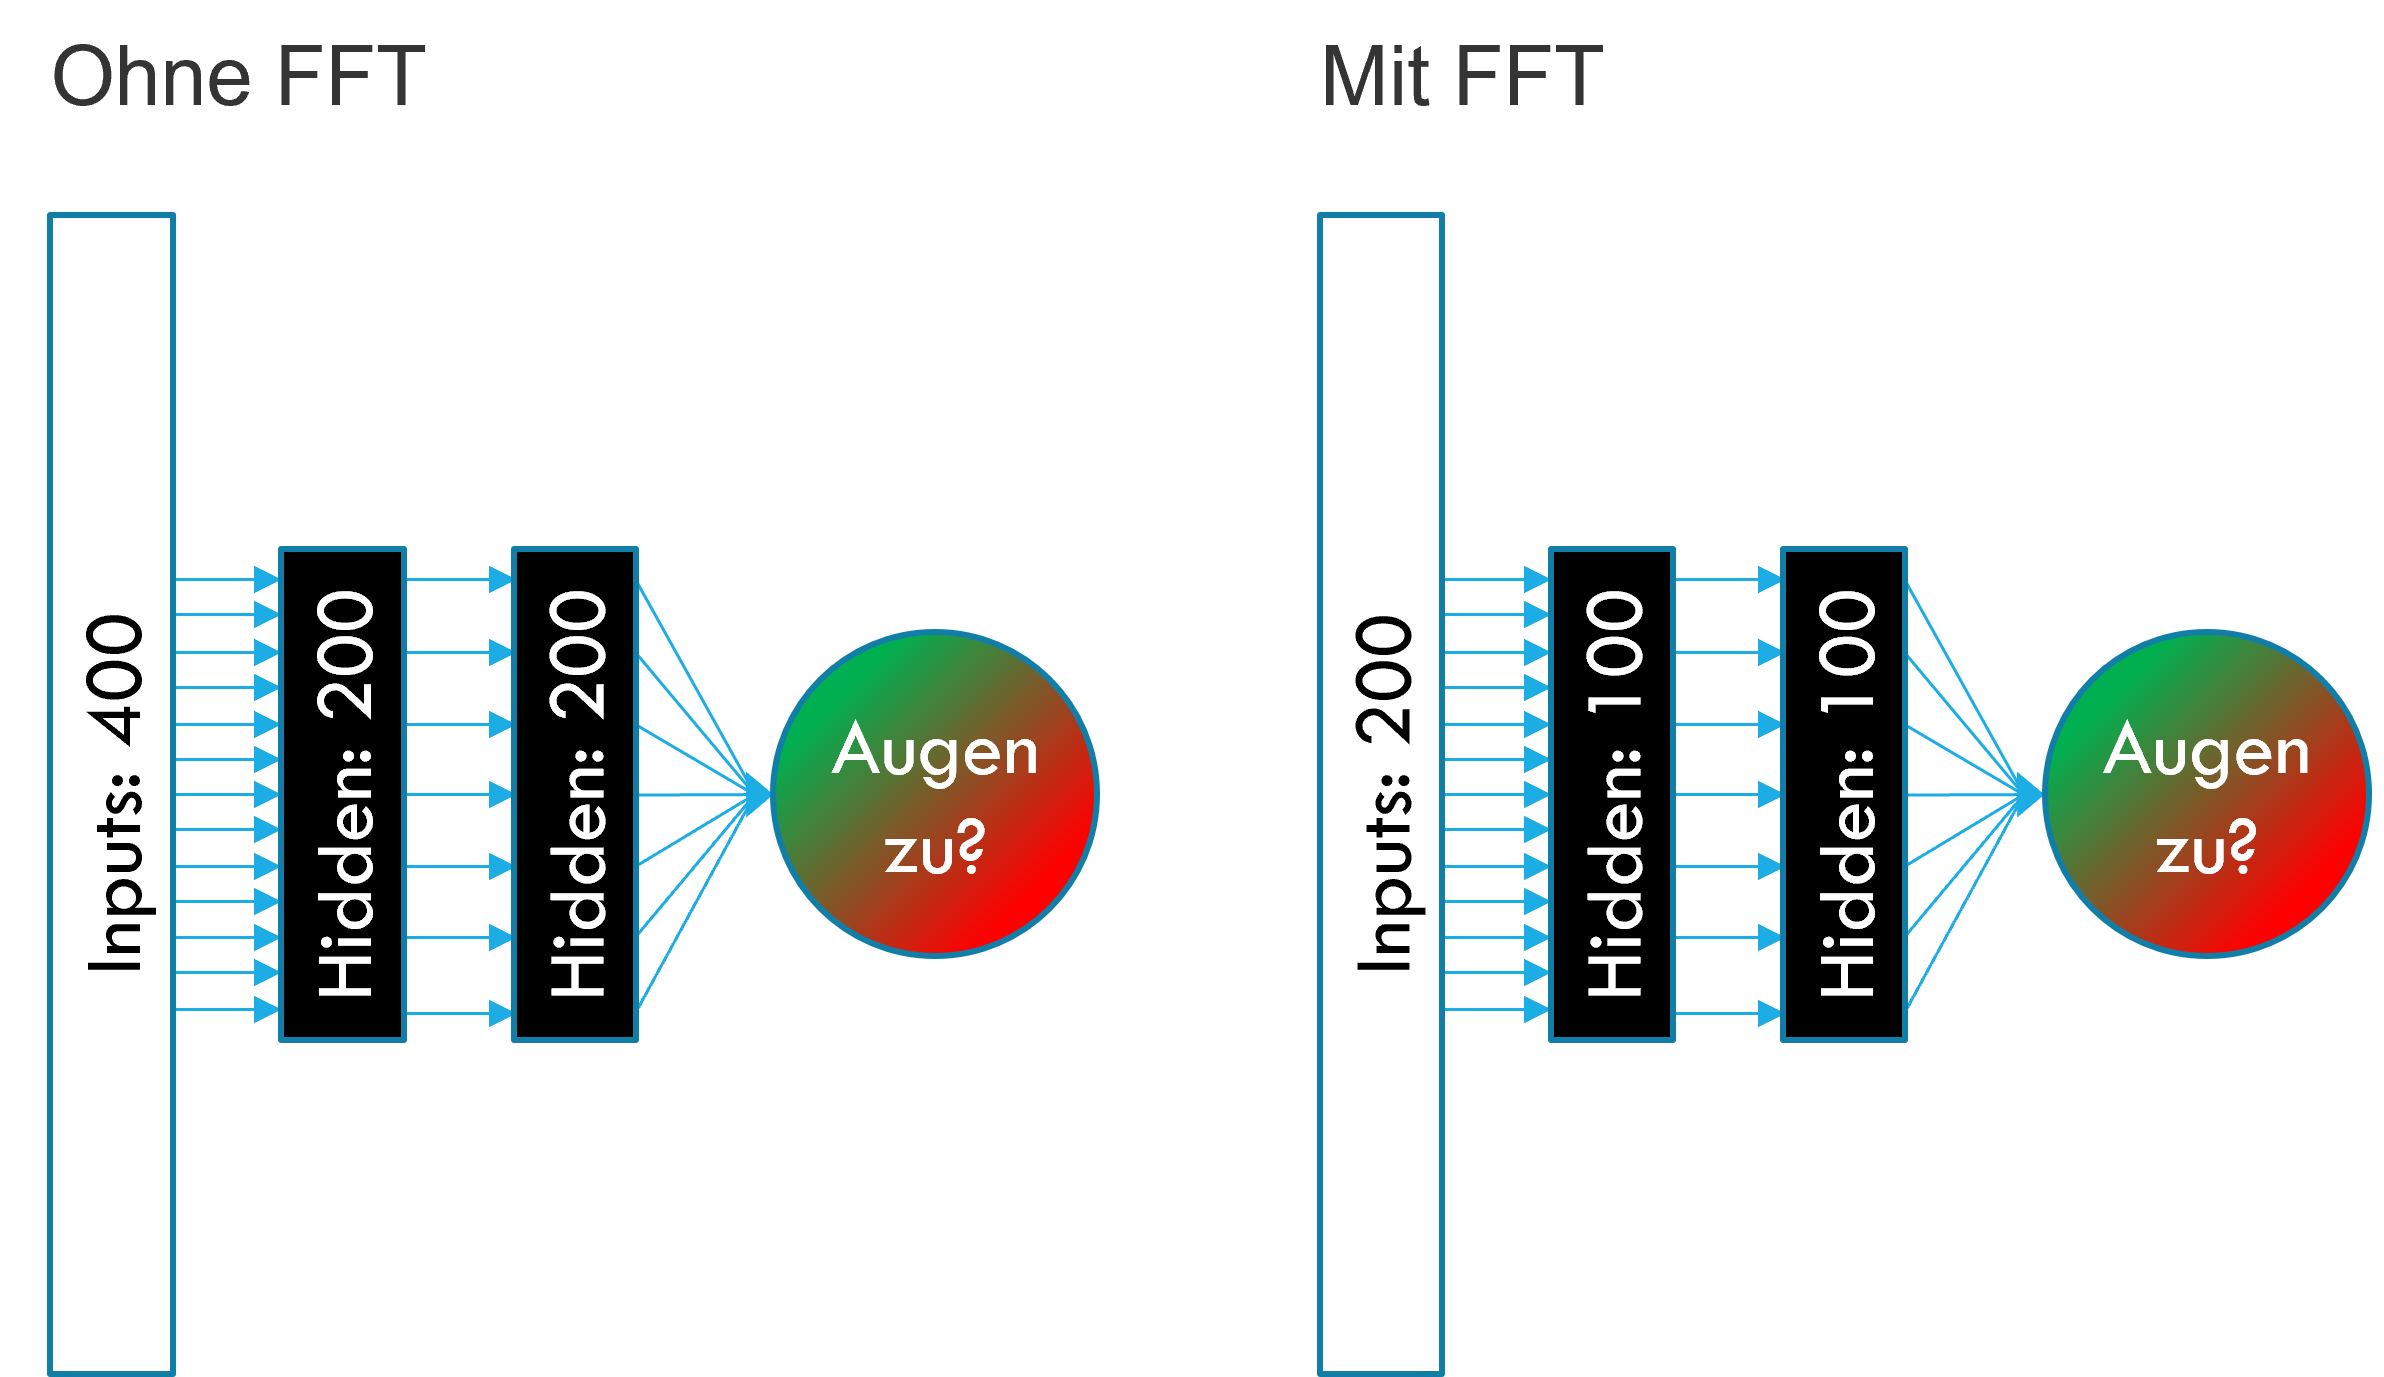
\includegraphics[width=0.7\textwidth]{pictures/netzwerkstruktur-emg.png}
		\caption{Struktur unseres neuronalen Netzwerks bei Verwendung von EMG (Konfiguration 1), links bei Vorverarbeitung mit FFT, rechts ohne. Mit FFT haben wir pro Elektrode nur 100 Inputs, da wir die Amplituden für Frequenzen 1-100 verwenden.}
		\label{emg-netzstruktur}}
	\end{figure}



	Nach diesem Erfolg gingen wir nun weiter zur Verwendung von EEG (Konfiguration 2). Dabei konnte das neuronale Netzwerk ebenfalls eine Testdaten-Genauigkeit von 95\% erreichen, jedoch nur mit FFT. Ohne FFT sah es deutlich schlechter aus (siehe Abbildung \ref{training2}): Die Genauigkeit mit den Trainingsdaten konnte zwar 100\% erreichen, jedoch blieb die Testdaten-Genauigkeit, welche viel repräsentativer für die Leistung bei der realistischen Verwendung ist, bei 47,5\% stehen.

	Der Grund dafür ist vermutlich ein Phänomen namens Überanpassung (overfitting). Dabei passt sich das neuronale Netzwerk zu stark an die Trainingsdatensätze an, wodurch das Netzwerk die Fähigkeit, auch neue, leicht unterschiedliche Daten korrekt zu erkennen, verliert / nicht erlernt. Dafür verantwortlich könnte sein, dass das Netzwerk zu lange trainiert wurde, oder was in unserem Fall wahrscheinlicher ist, ohne FFT keine tieferen Zusammenhänge finden konnte.

	\begin{figure}[H]
		\fig{
		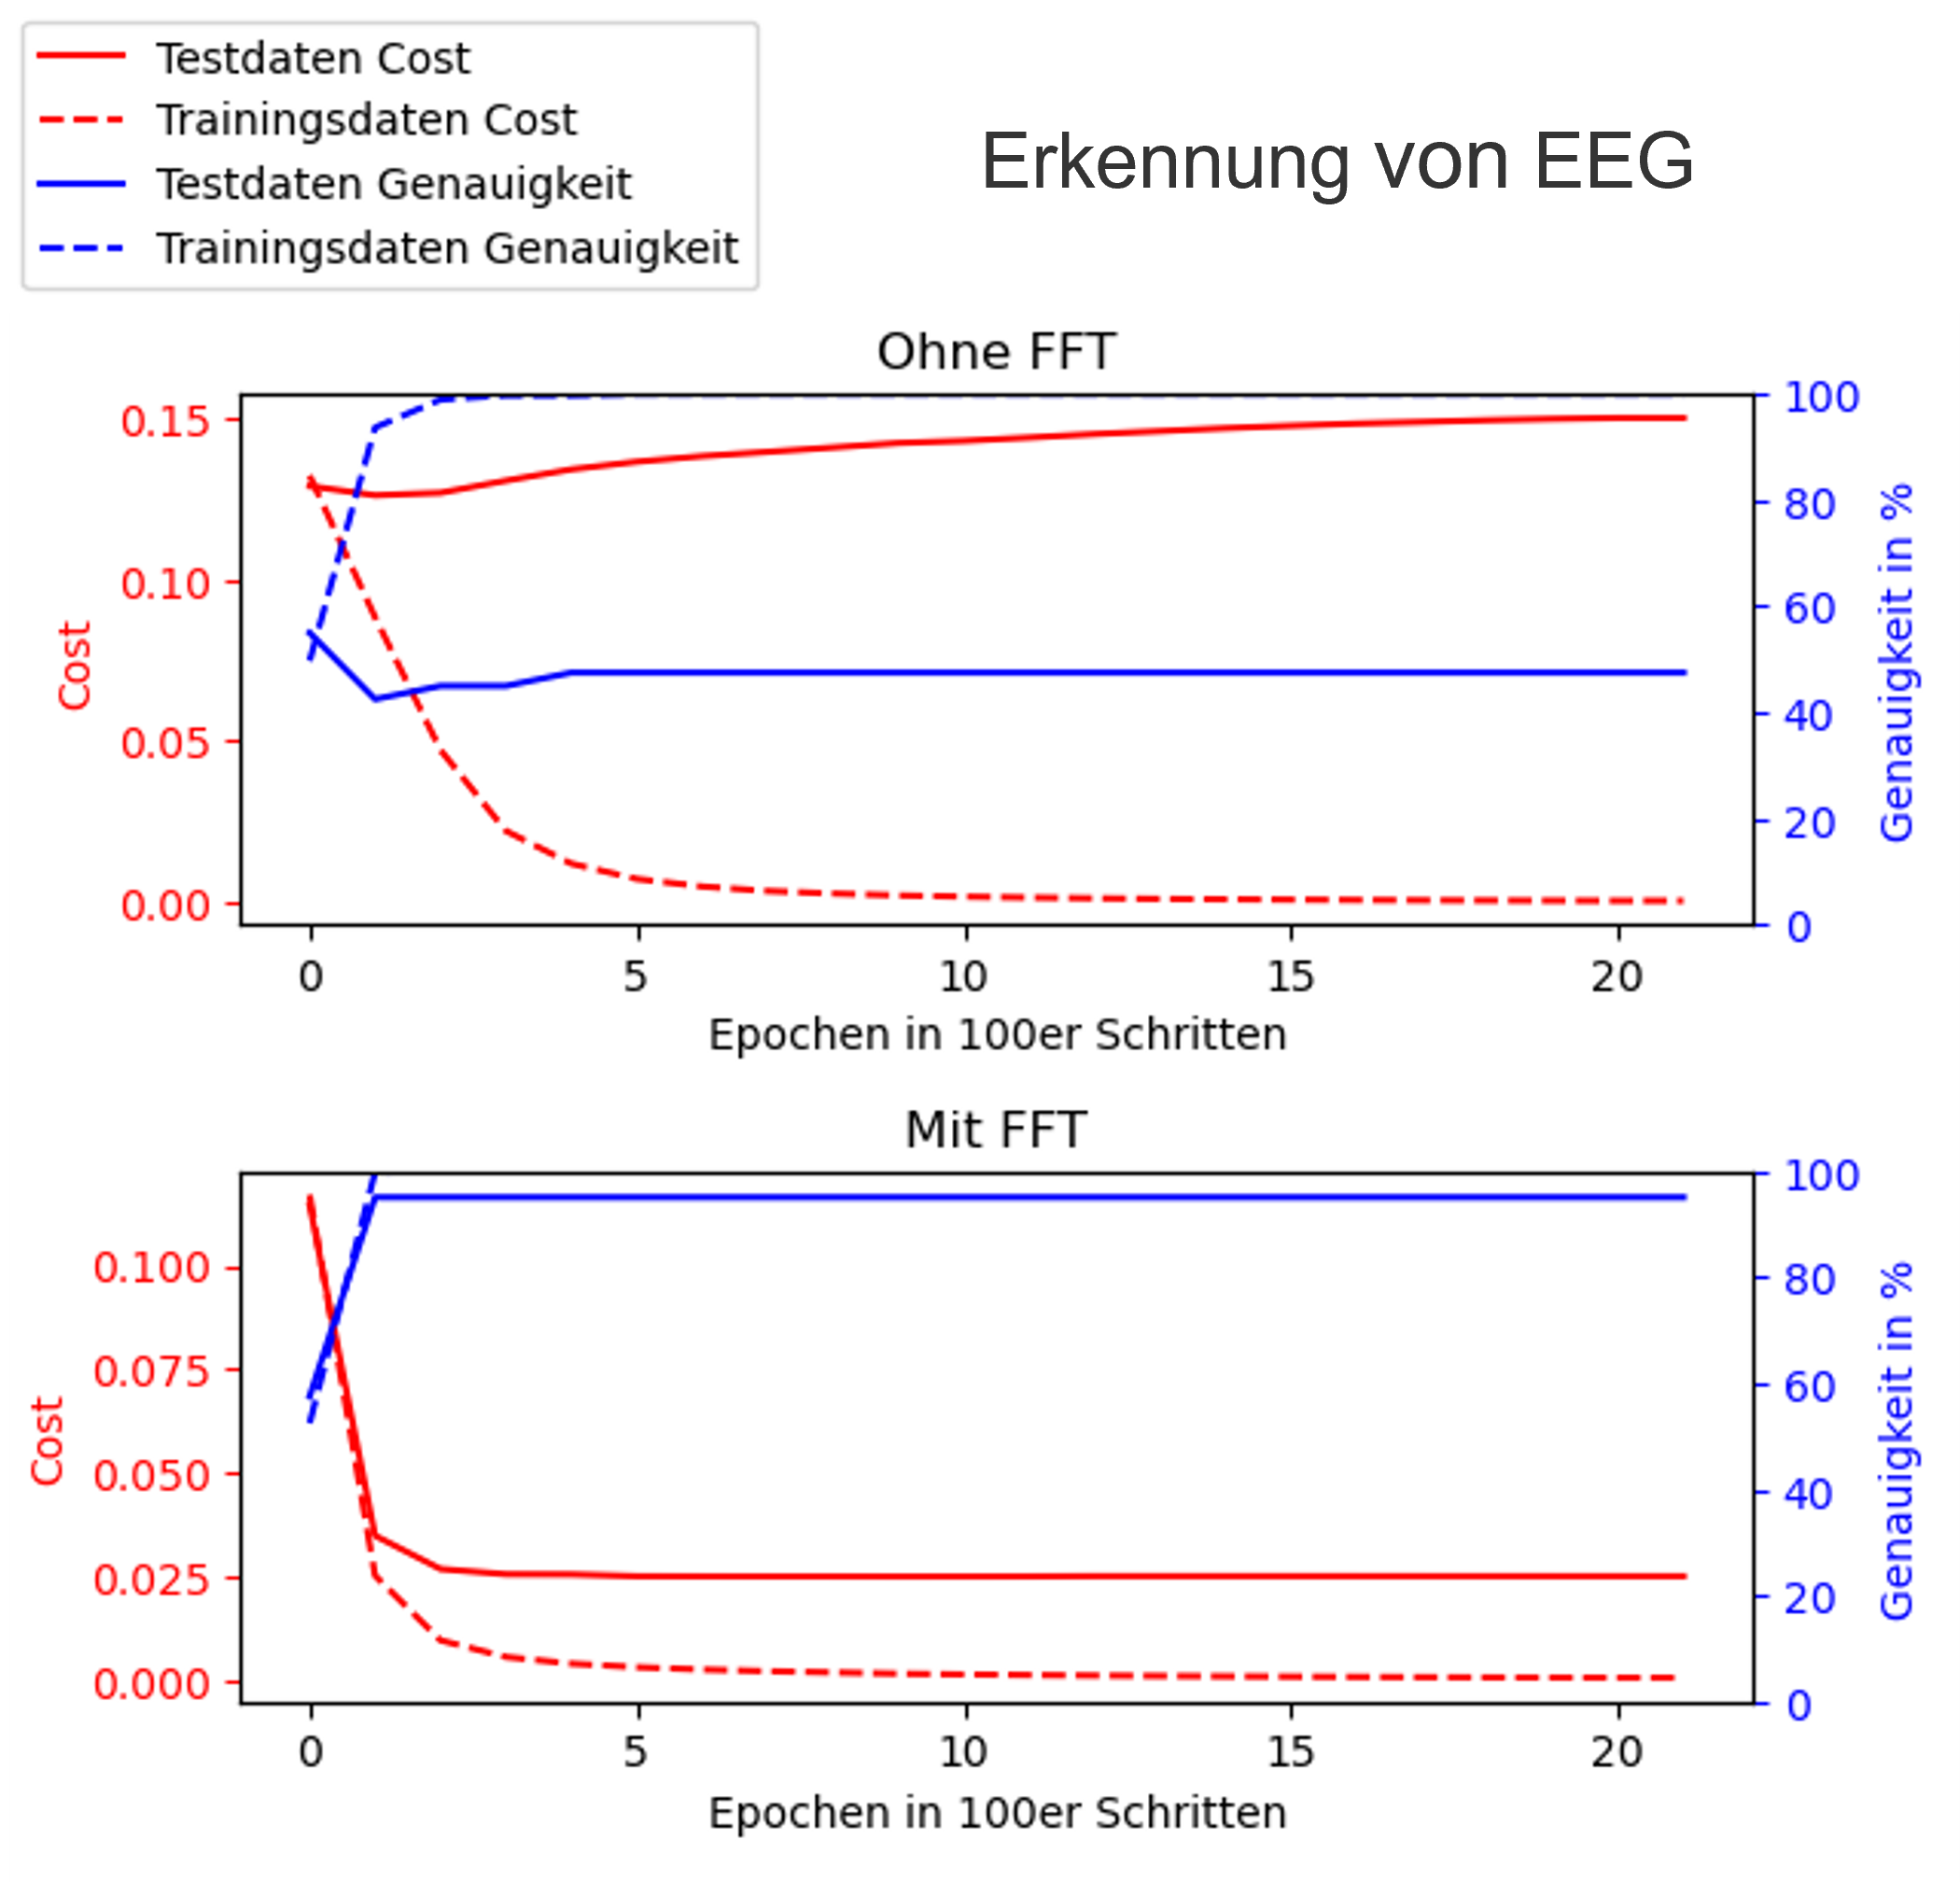
\includegraphics[width=0.7\textwidth]{pictures/Trainingsprozess_EEG_FFT_vs_kein_FFT2.png}
		\caption{Es wurde EEG benutzt. Zu sehen ist der Cost- und Genauigkeitsverlauf der Test- und Trainingsdaten beim Trainieren des Netwerkes, oben ohne Vorverarbeitung durch FFT und unten mit. Eine Epoche entspricht jeweils einer Backpropagation mit allen Trainings-Datensätzen.}
		\label{training2}}
	\end{figure}

	Ein Live-Test mit FFT verlief gut, wie man in der Aufnahme dessen sehen kann. \cite{projekt-video2}
%
	Die Netzwerkstruktur für EEG ist in Abbildung \ref{eeg-netzstruktur} zu sehen.

	Der gesamte Quellcode unseres Projektes ist auf unserem GitHub Repository \enquote{Interpreting-EEG-with-AI} veröffentlicht. \cite{InterpretingEEG}

	\begin{figure}[H]
		\fig{
		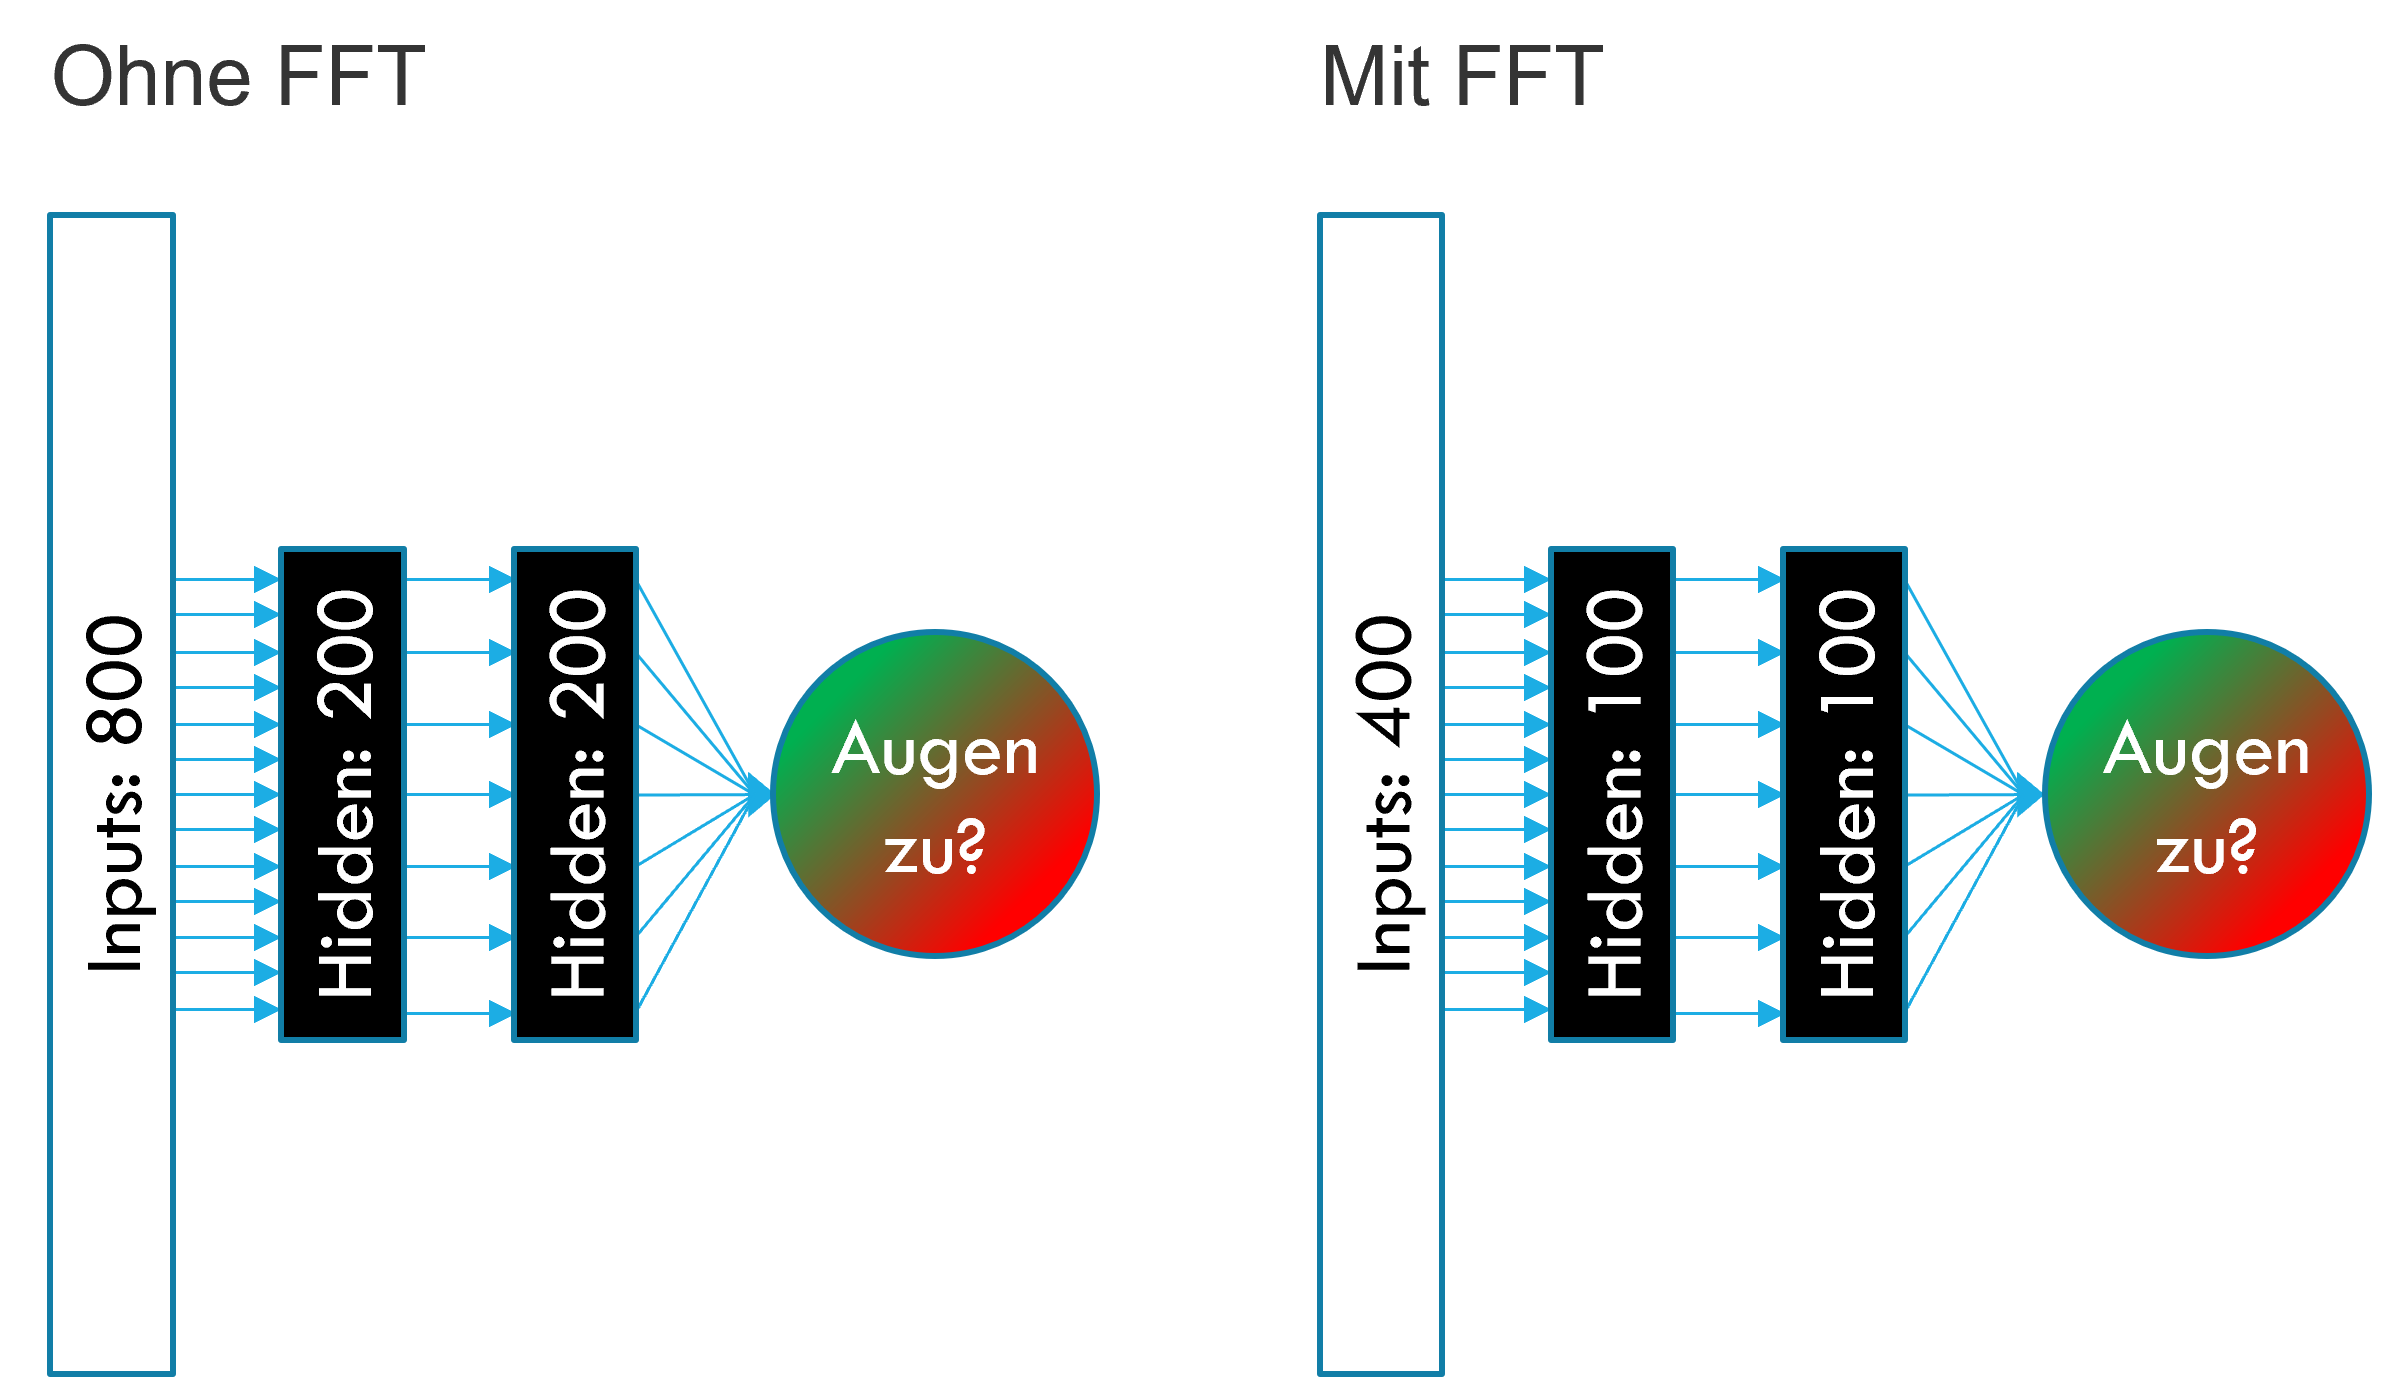
\includegraphics[width=0.7\textwidth]{pictures/netzwerkstruktur-eeg.png}
		\caption{Struktur unseres neuronalen Netzwerks bei Verwendung von EEG (Konfiguration 2), links bei Vorverarbeitung mit FFT, rechts ohne. Mit FFT haben wir pro Elektrode nur 100 Inputs, da wir die Amplituden für Frequenzen 1-100 verwenden.}
		\label{eeg-netzstruktur}}
	\end{figure}

	\section{Diskussion}

	Wir sind zufrieden damit, dass wir unser erstes Teilziel erreicht haben: Der Roboter fährt sicher, und es gibt kaum eine Verzögerung. Die Kosten der benutzten Hardware halten sich noch in Grenzen: Beim Kauf hat die gesamte EEG-Ausstattung ca. 550€ gekostet, was zwar eigentlich eine hohe Summe ist (danke an den Förderverein für die Finanzierung!), aber professionelle Ausrüstung kostet deutlich mehr. Die Performance des Programms kann außerdem zwar noch verbessert werden, jedoch dauern beim Trainieren 1000 Epochen (genug für ca. 100\% Genauigkeit) auf dem Test-System bereits lediglich 5 Minuten. 

	Als Nächstes wollen wir unser Programm auch mit Personen testen, von denen wir vorher keine Trainingsdaten gesammelt haben.
%
	Danach wird das Ziel sein, auf andere EKPs wie Konzentration umzusteigen, und vielleicht sogar mehrere gleichzeitig zu erkennen, damit wir für den Roboter mehr \enquote{Kontrolldimensionen} haben können, z.B. für Geschwindigkeit, rechts / links, etc. Wenn wir genügend EKPs sicher erkennen können, dann könnten wir sogar die Steuerung einer Drohne versuchen. Man könnte dafür auch für mehrere Befehle ein EKP nutzen. Z.B. könnte zweimal schnell hintereinander Blinzeln für rechts, dreimal für links, viermal für oben, etc. stehen. Man könnte für eine Texteingabe auch versuchen, \enquote{Protokolle} wie Morsecode zu erkennen. Für eine korrekte Klassifizierung eines einzelnen Ereignisses (z.B. Augenschließen) braucht unser System eine Sekunde. Das heißt, wir könnten Signale mit einer Datenübertragungsrate von 1 Bit pro Sekunde verarbeiten.

	Ein Problem, welches wir hatten, war unsere EEG-Messausrüstung. Sie war sehr anfällig für Störungen: Die Kabel durften nicht berührt werden, nicht zu viele technische Geräte durften in der Nähe sein, und in einigen Räumen war die Signalqualität manchmal sehr stark gestört, ohne dass wir wussten, warum. Also wollen wir mögliche Störfaktoren finden und eliminieren, damit wir konsistente Ergebnisse haben können.

	Außerdem wollen wir uns einen Raspberry Pi 4B mit 8\,GB Arbeitsspeicher besorgen. Dieser sollte leistungsfähig genug sein, um unser Programm auch direkt auf dem Roboter ausführen zu können. So wären das EEG-Gerät und der Roboter auch ohne einen extra Laptop nutzbar.

	%	Weiter sind uns bei unseren Fourier-Analysen zwei Dinge aufgefallen:
	%
	%	Erstens erhalten wir immer sehr hohe Amplituden. Sie sind zwar proportional zu dem, was man erwarten würde, und somit sollte dies die Leistung des neuronalen Netzwerkes nicht beeinflusst haben, jedoch würden wir trotzdem gerne die Ursache finden und das Problem beheben. 
	%
	%	Zweitens sind 
	
	Eine weitere Verbesserungsmöglichkeit sehen wir in der Fourier-Analyse:
	Bei unserem aktuellen Aufbau sind vor allem die niedrigen Frequenzen wichtig, da wir die Alpha-Blockade zur Erkennung nutzen und am Okzipitalen Kortex die Alpha-Wellen dominant sind. Die Bedeutung des niedrigen Frequenzbereichs kann man auch in Abbildung \ref{EEG-FFT} sehen. Es könnte sich also lohnen, z.B. nur die Amplituden der Frequenzen 1-20 Hertz an das neuronale Netz als Inputs zu geben, um die Leistung und Performance des neuronalen Netzes weiter zu steigern. 

	\newpage

	\section{Danksagung}

	\subsection{Finanzierung} \label{Foerderverein}

	Danke an den Förderverein \enquote{Gesellschaft der Freunde des Gymnasium Eversten e.V.} für die Finanzierung des EEG-Geräts. Alle finanzierten Teile sind in der \hyperref[Materialien]{Materialliste} mit $\star$ gekennzeichnet. 

	\subsection{Unterstützung} \label{Unterstuetzung}

	Vielen Dank an Professor Everling vom \enquote{The Brain and Mind Institute} der Western University in Kanada \footnote{\url{https://www.uwo.ca/bmi/investigators/stefan-everling.html}}, der uns in einem Gespräch mit ihm geholfen hat, einen Ansatz in diesem komplizierten Thema zu finden, und praktische Tipps zum Umgang mit dem EEG gegeben hat.

	Dank geht auch an Ino Saathoff, der für uns die Hülle der EEG-Platine mit seinem 3D-Drucker erstellt hat.

	Wir danken ebenfalls Oliver Samkovskij, der die Lego-Struktur des Roboters gebaut hat, und Ino, der für die Verkabelung und Stromversorgung verantwortlich war. Der Roboter ist zwar mit viel mehr ausgestattet als für unser Projekt notwendig, aber dank euch mussten wir nicht unnötig einen neuen bauen.

	\section{Quellen \& Referenzen}

	\subsection{Abbildungen}

	Die Vorlage des 10-20-Systems, welche wir in Abbildung \ref{10-20-System} verwendet haben, stammt von \url{https://en.wikipedia.org/wiki/File:21_electrodes_of_International_10-20_system_for_EEG.svg} und liegt in der Public Domain.
	
	Alle anderen Abbildungen und Fotos wurden von uns selbst erstellt.

	\subsection{Literatur}
	\printbibliography[heading=none, keyword={Literatur}, notkeyword={YTVideos}]

	\subsection{Videos}
	\printbibliography[heading=none, keyword={YTVideos}]

	\subsection{Programme}
	\printbibliography[heading=none, keyword=Programme]

\end{document}